\documentclass[12pt,a4paper]{beamer}
\usetheme{Amsterdam}
%\usecolortheme{beaver}
\usepackage[english,french]{babel}
\usepackage{graphicx}
%\usepackage[utf8]{inputenc}  
\usepackage[T1]{fontenc}
\usepackage{fontspec}
\usepackage{amsmath}
\usepackage{amsfonts}
\usepackage{amssymb}
\usepackage{tikz}
\usepackage{listings}
\usepackage{pgfplots}
%\pgfplotsset{compat=1.14}
\pgfplotsset{compat=newest}

\usepackage{color}

\usepackage{color}
\definecolor{mygreen}{rgb}{0,0.6,0}
\definecolor{mygray}{rgb}{0.5,0.5,0.5}
\definecolor{mymauve}{rgb}{0.58,0,0.82}
\definecolor{greenfluo}{rgb}{0,255,0}
\definecolor{blueemph}{RGB}{17,59,94}

%Underline in color
\newcommand{\coloruline}[3]{\emph{\textcolor{#1}{\underline{#2\textcolor{black}{#3}}}}}

%
\setbeamertemplate{blocks}[rounded]
%\renewcommand{\insertnavigation}[1]{}
\def\insertnavigation#1{\relax}




\lstset{
  language=Java,
  commentstyle=\color{mygreen},    % comment style
  stringstyle=\color{mymauve},     % string literal style
  keywordstyle=\color{blue},       % keyword style
  basicstyle=\footnotesize        % the size of the fonts that are used for the code
}

\title{\textbf{Algorithmique avancée}}
\subtitle{Piles et Files}
\author{Frédéric Guyomarch}
\date{2018/2019 - Semestre 3}
\institute % (optional)
{

  Université de Lille1\\
  IUT-A de Lille

}
 

 
\logo{
\includegraphics[width=5em]{figs/iutaustl}}

%Remove Figure prefix on captures
\setbeamertemplate{caption}{\raggedright\insertcaption\par}

%Remove Control bar
\beamertemplatenavigationsymbolsempty





\begin{document}

\begin{frame}
\titlepage
\end{frame}

\begin{frame}{Introduction}
\begin{itemize}
\item Structures de données différentes
\item Tableaux, listes : stockage + accès 
\item Piles/files : structures conceptuelles
\item Structures abstraites et accès restreint
\end{itemize}




\end{frame}

\begin{frame}{Plan}
\tableofcontents
\end{frame}

\section{Piles}

\begin{frame}{Des Piles, pourquoi?}
Quelques exemples d'utilisation:
\begin{itemize}
\item Recherche de chemins (labyrinthe) 
\item Gestion d'un historique de modifications (fonctions undo/redo)
\item Gestion de la récursivité dans un langage (pile d'appels)
\end{itemize}

\end{frame}

\begin{frame}{Pile}{}
\begin{itemize}
\item Une pile est un conteneur d'éléments qui respecte le principe du \textcolor{blueemph}{\textit{Last In First Out}} (LIFO): le premier élément accessible est le dernier ajouté.
\item On ne peut accéder qu'à l'élément placé au sommet de la pile.
\item Un distributeur de PEZ$^{\mbox{\scriptsize{\textregistered}}}$ en est un bon exemple:
\end{itemize}
\begin{figure}
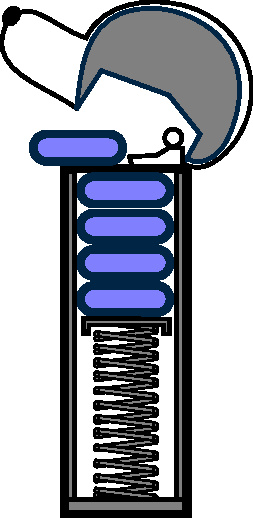
\includegraphics[scale=0.4]{figs/pez}
\end{figure}

\end{frame}



\begin{frame}{Pile: LIFO}{}
\only<1>{
Pile à l'origine, 10 est la valeur au sommet:
\begin{figure}
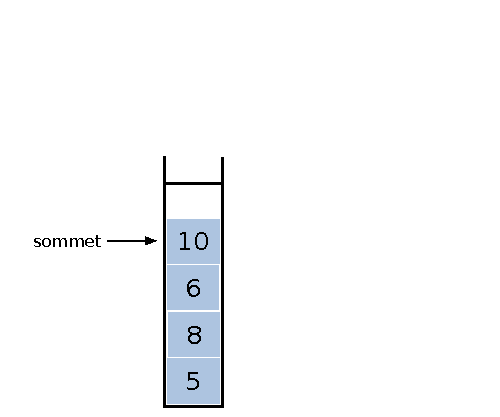
\includegraphics[scale=0.9]{figs/stack}
\end{figure}
}

\only<2>{
On dépile 10 (retire la valeur 10 au sommet):
\begin{figure}
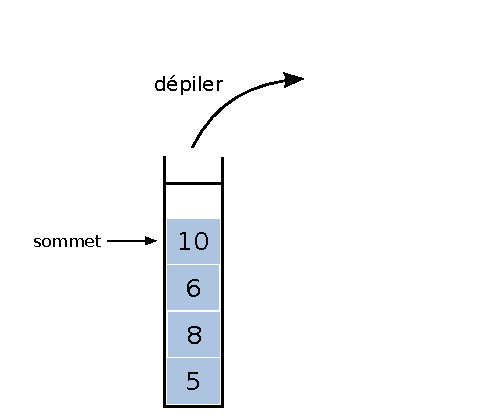
\includegraphics[scale=0.9]{figs/stack_pop1}
\end{figure}
}

\only<3>{
6 devient la valeur au sommet de la pile:
\begin{figure}
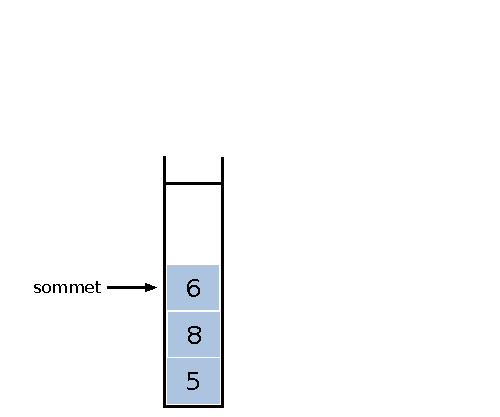
\includegraphics[scale=0.9]{figs/stack_pop2}
\end{figure}
}

\only<4>{
On empile 14 (ajoute la valeur 14 au sommet):
\begin{figure}
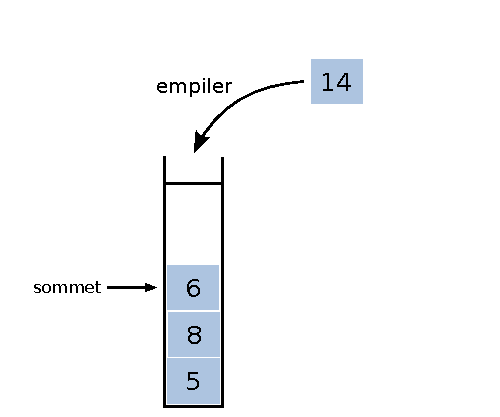
\includegraphics[scale=0.9]{figs/stack_push1}
\end{figure}
}

\only<5>{
Le sommet de la pile est 14:
\begin{figure}
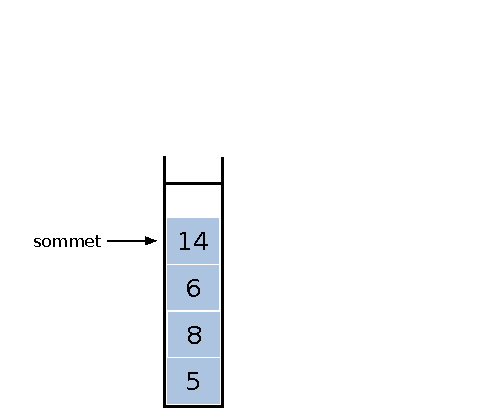
\includegraphics[scale=0.9]{figs/stack_push2}
\end{figure}
}
\end{frame}

\begin{frame}{TDA Pile}{Opérations}
Le type de données abstrait Pile spécifie plusieurs opérations principales:
\begin{itemize}
\item \texttt{empiler(T val)}: Empile une valeur de type T
\item \texttt{T dépiler()}: Dépile une valeur
\item \texttt{T sommet()}: Retourne (sans la retirer) la valeur au sommet de la pile
\item \texttt{boolean estVide()}: teste si la pile est vide
\end{itemize}

\end{frame}


\begin{frame}{Pile}{Application: \textcolor{blueemph}{Parcours en profondeur}}

\only<1>{
\begin{figure}
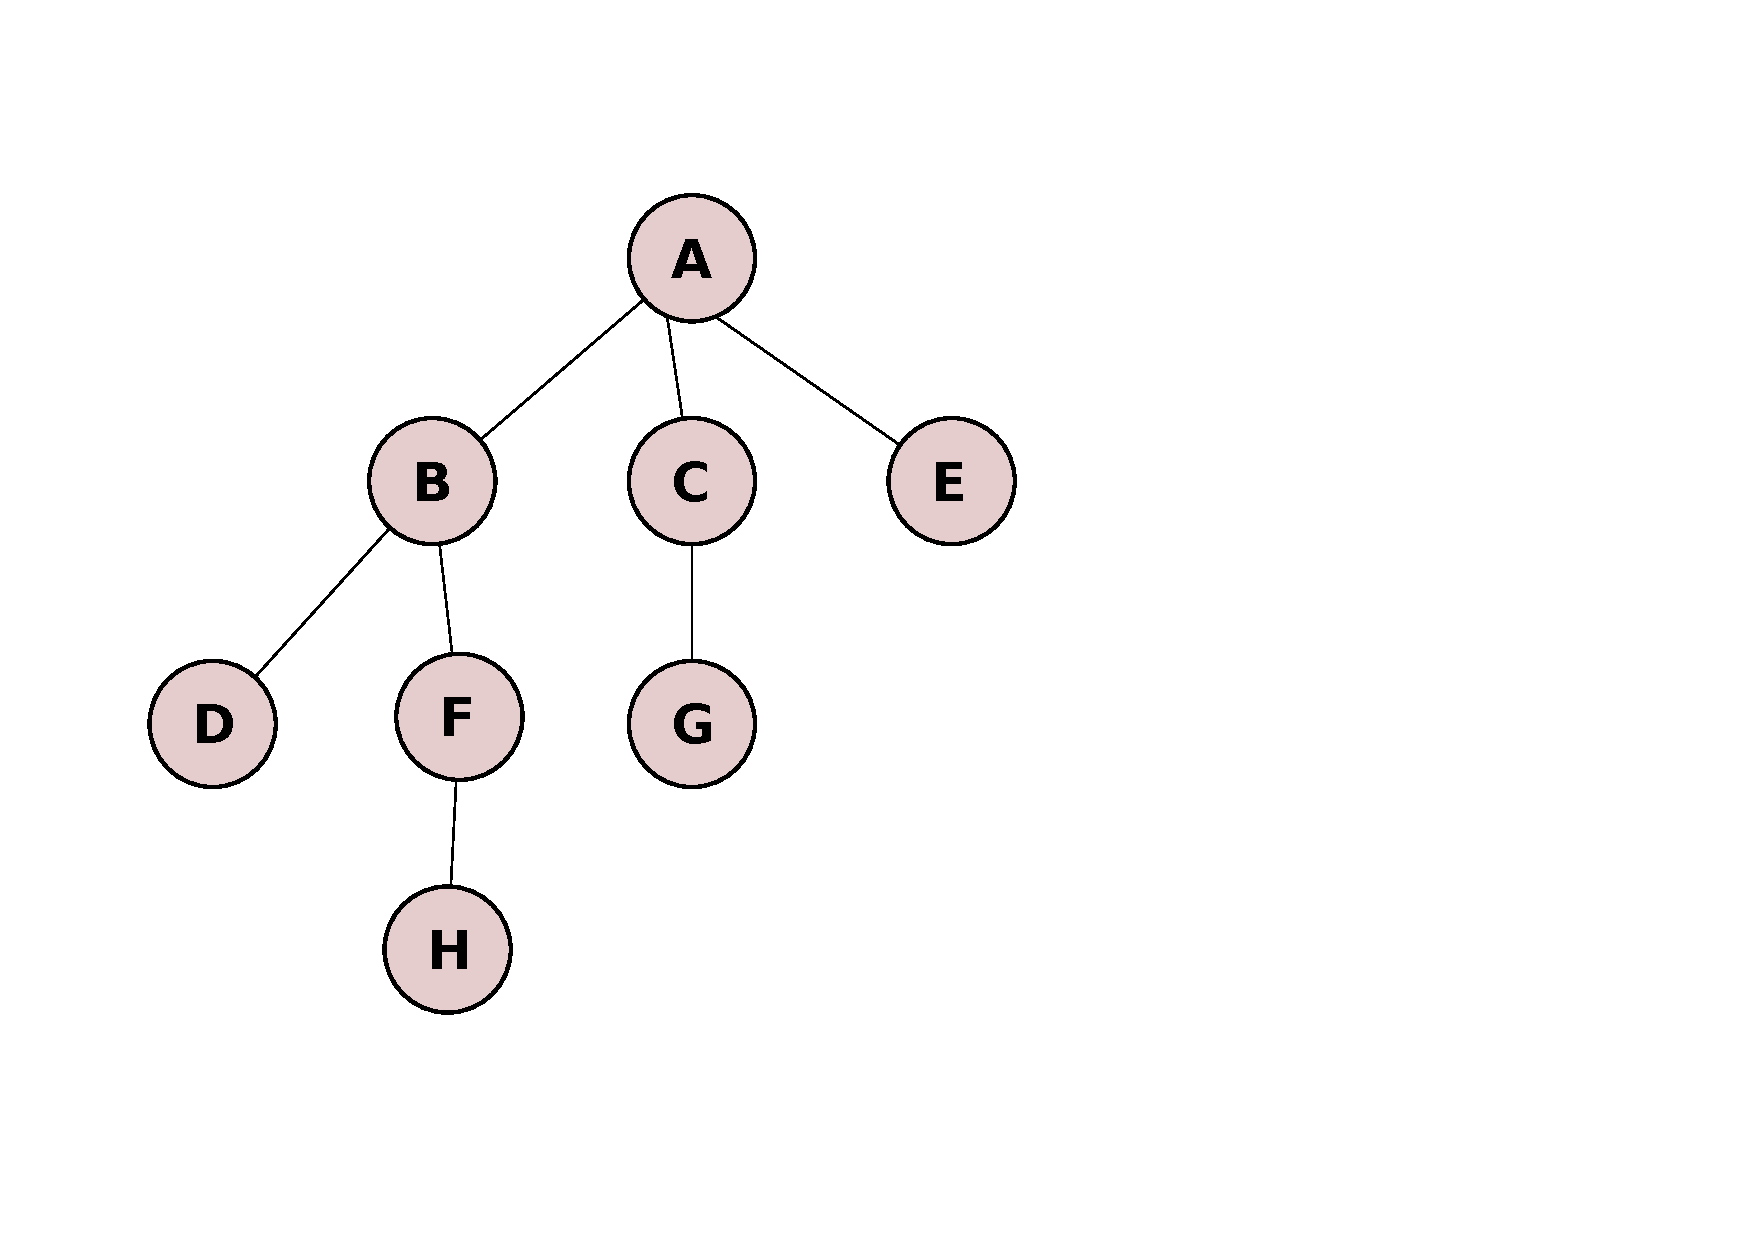
\includegraphics[scale=0.35]{figs/graph}
\end{figure}
}

\only<2>{
\begin{figure}
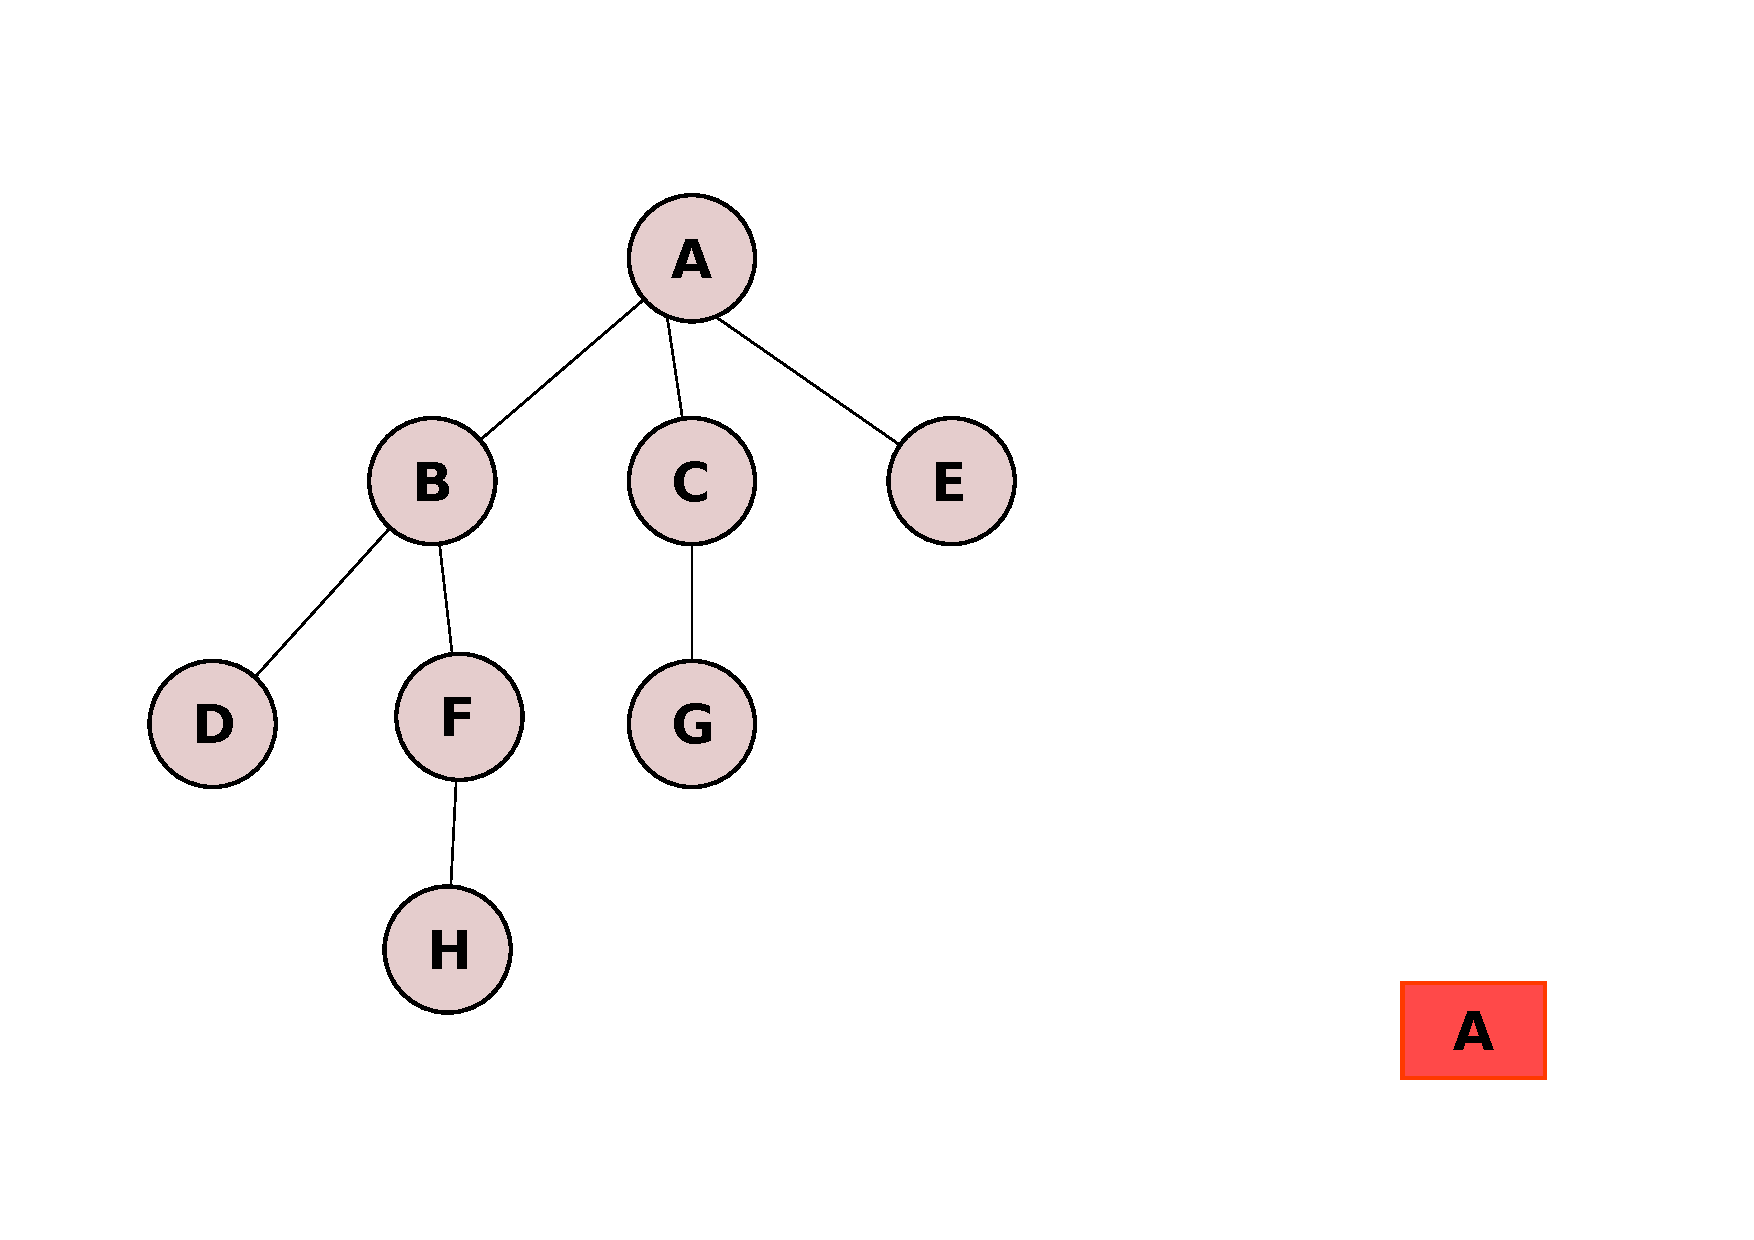
\includegraphics[scale=0.35]{figs/graph_dfs_A}
\end{figure}
}

\only<3>{
\begin{figure}
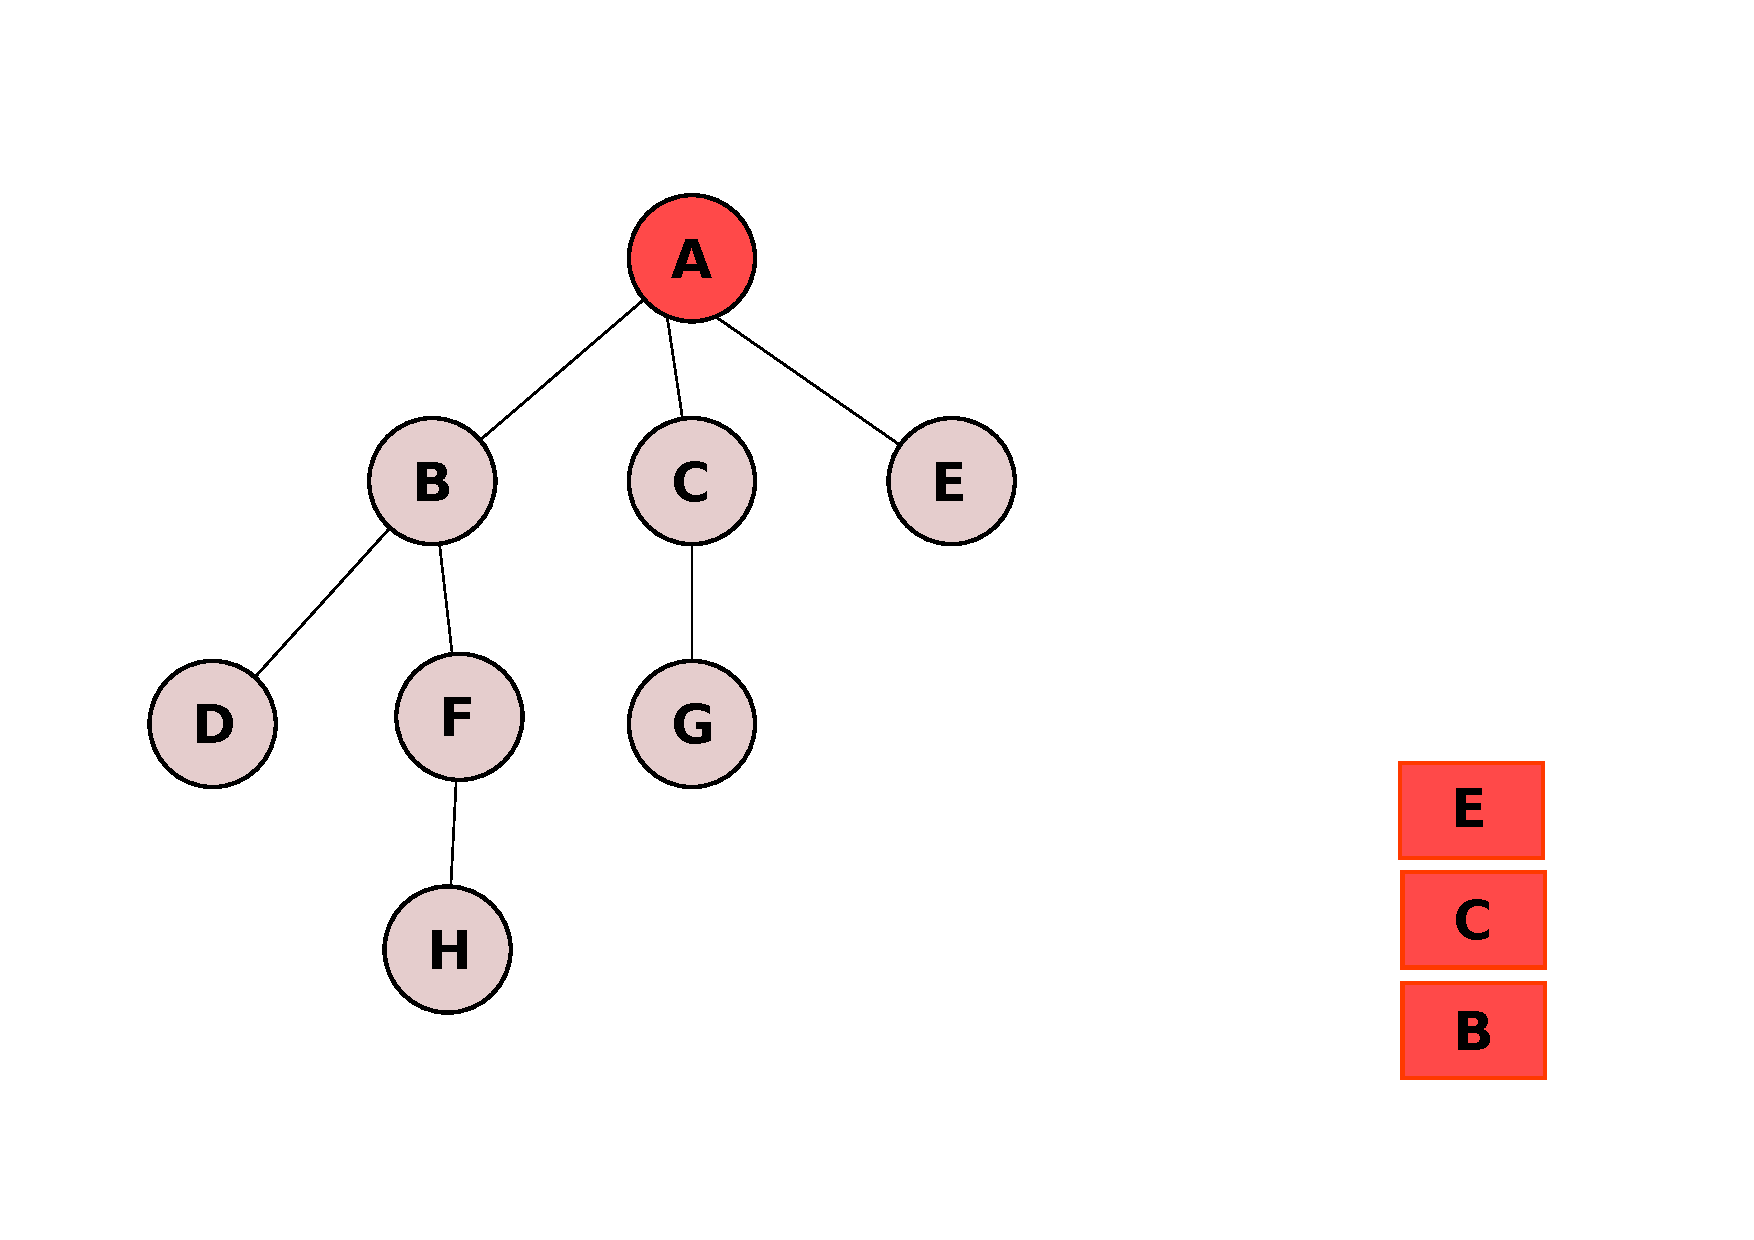
\includegraphics[scale=0.35]{figs/graph_dfs_BCE}
\end{figure}
}

\only<4>{
\begin{figure}
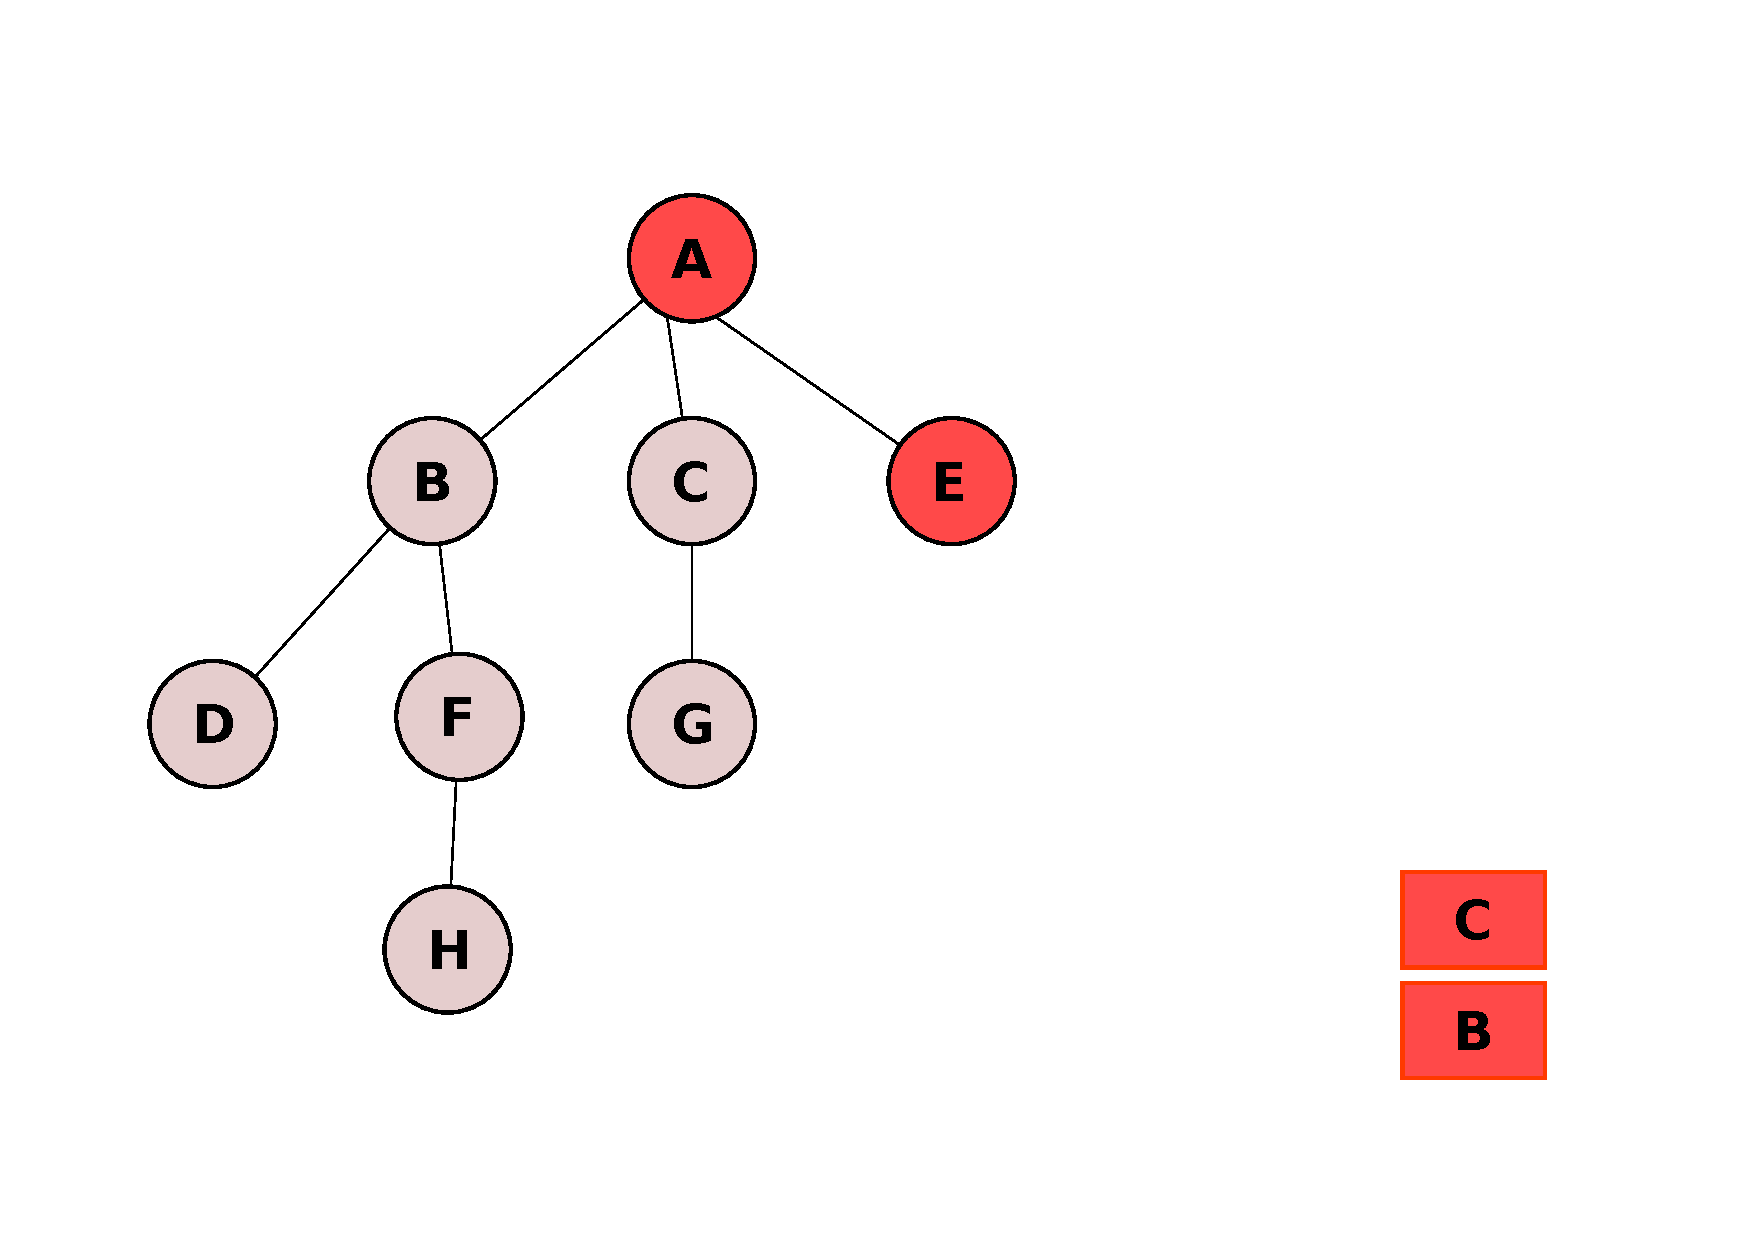
\includegraphics[scale=0.35]{figs/graph_dfs_BC}
\end{figure}
}

\only<5>{
\begin{figure}
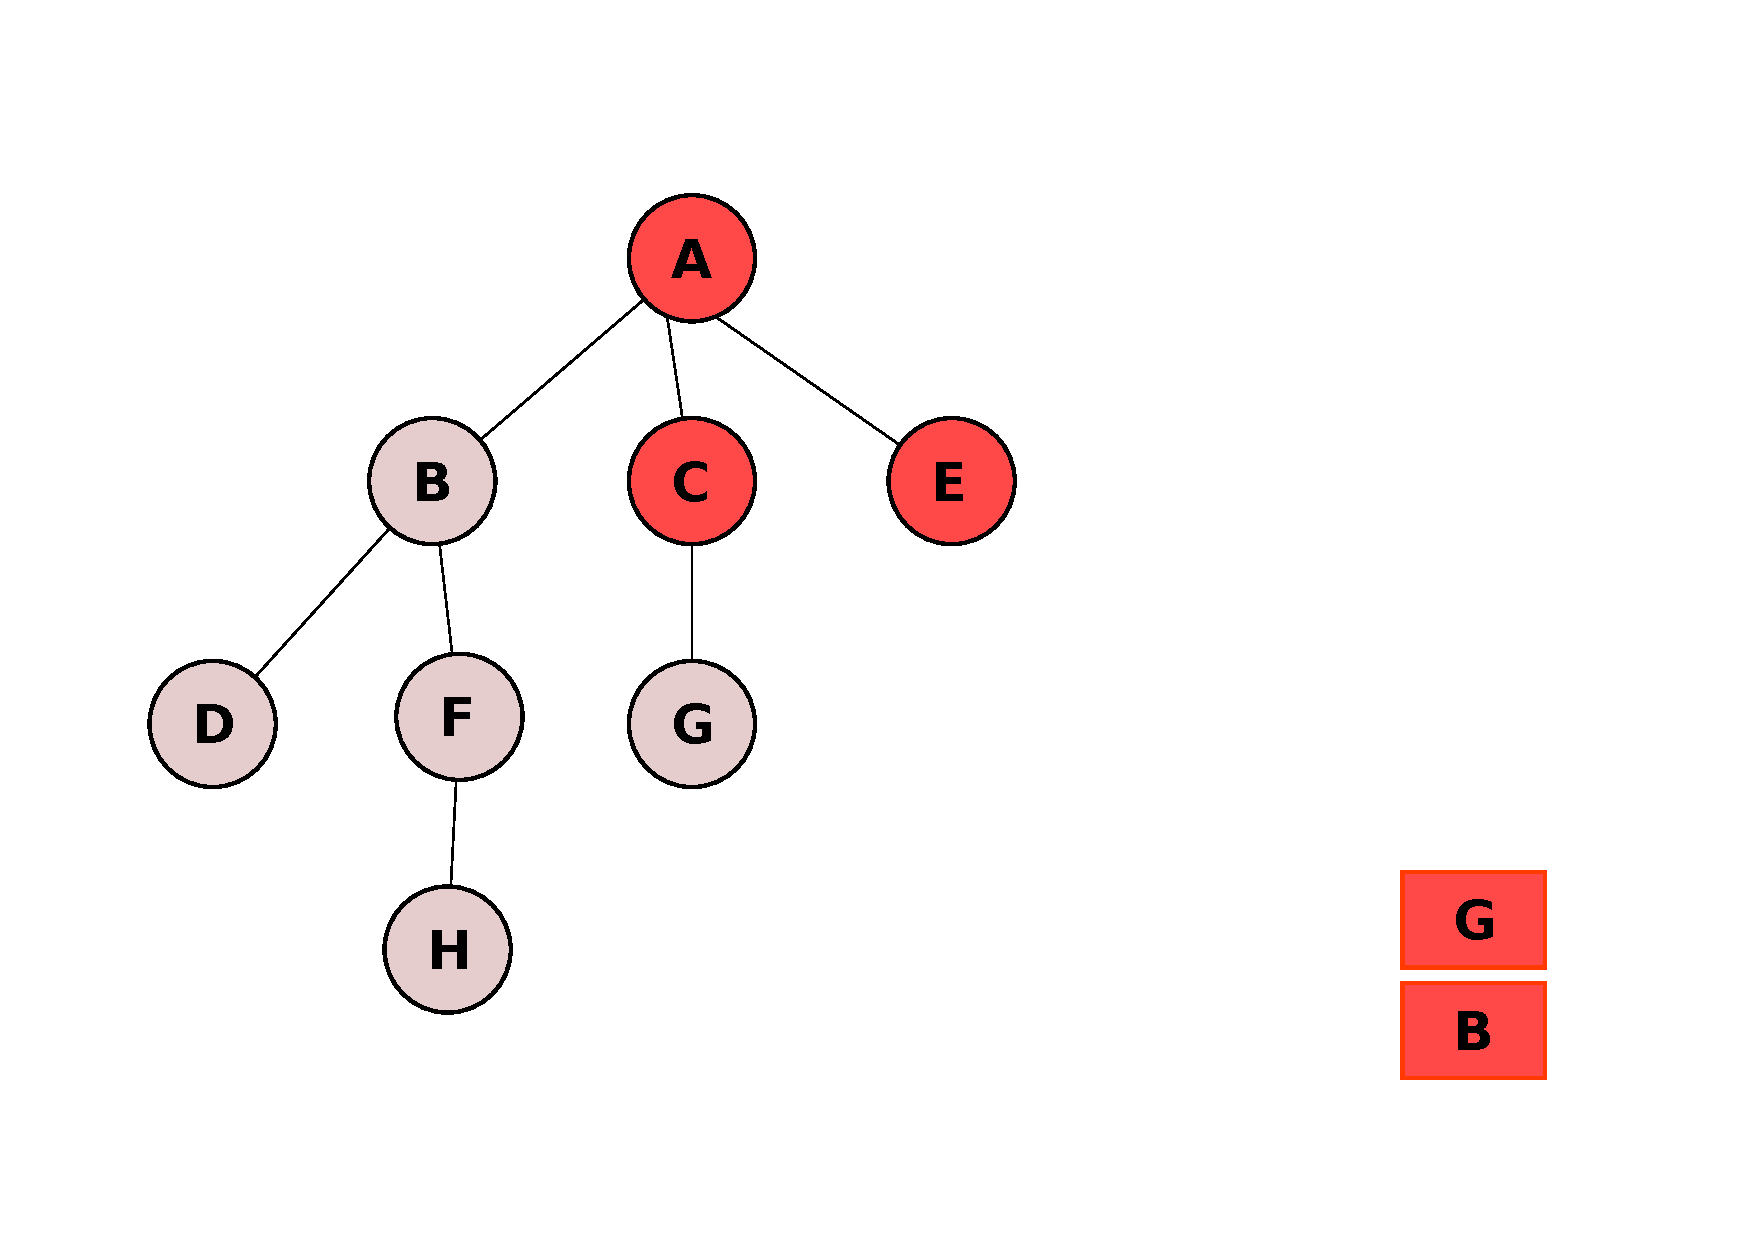
\includegraphics[scale=0.35]{figs/graph_dfs_BG}
\end{figure}
}

\only<6>{
\begin{figure}
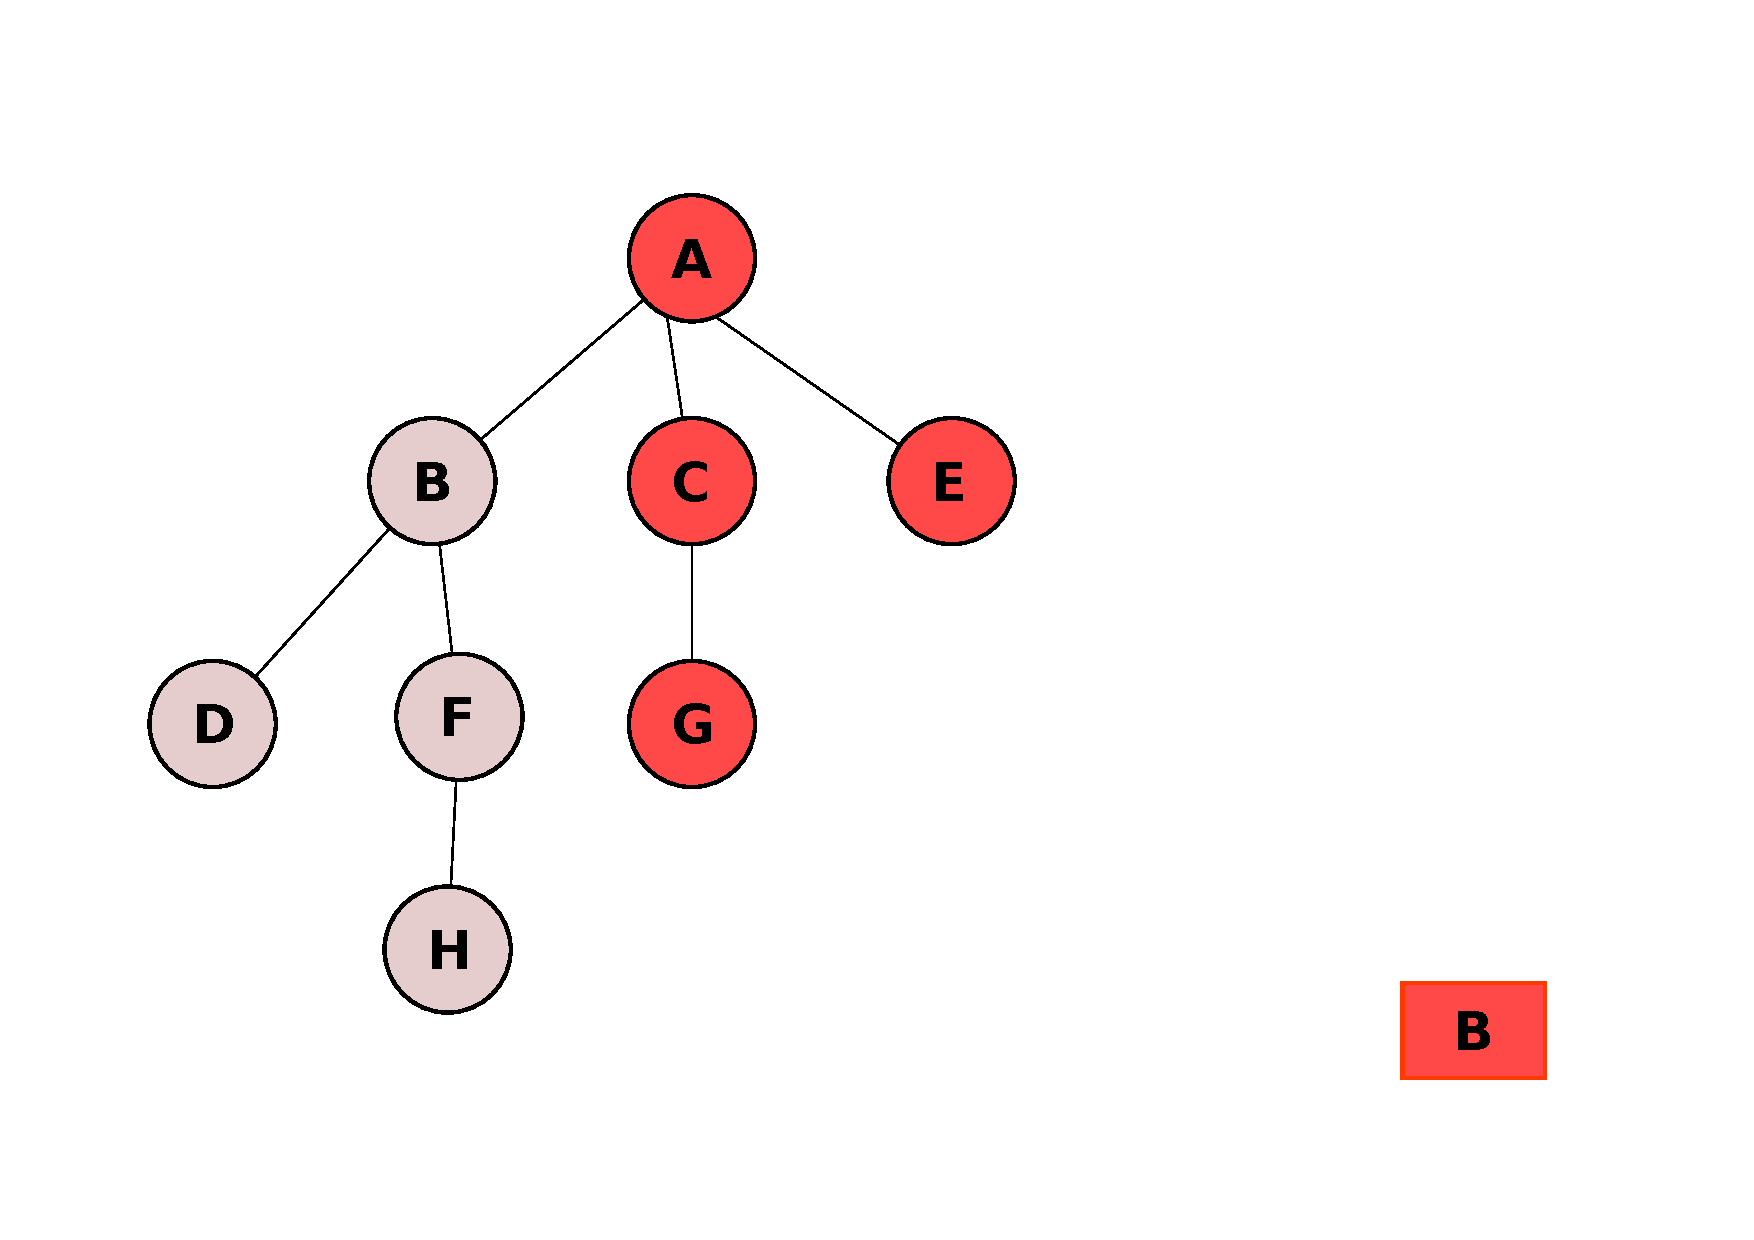
\includegraphics[scale=0.35]{figs/graph_dfs_B2}
\end{figure}
}
\only<7>{
\begin{figure}
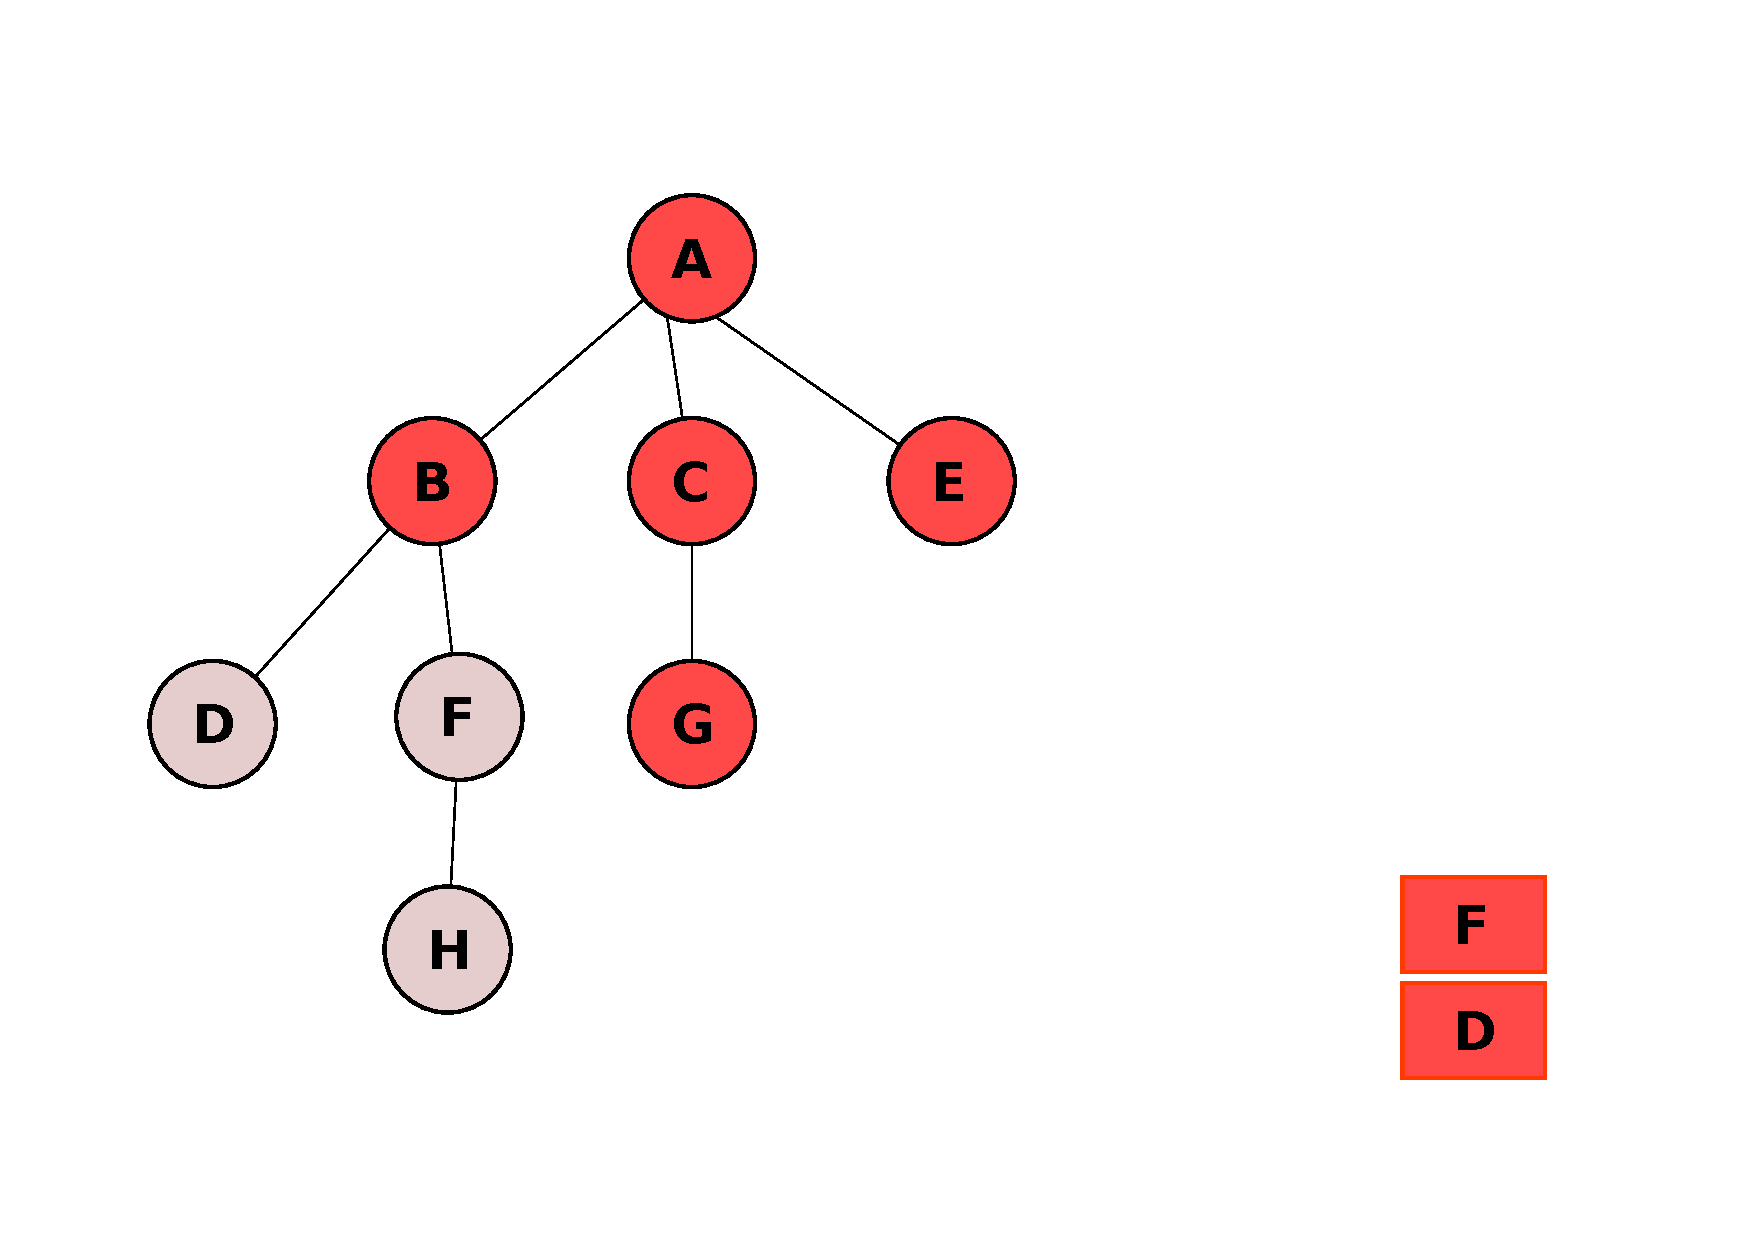
\includegraphics[scale=0.35]{figs/graph_dfs_FD}
\end{figure}
}
\only<8>{
\begin{figure}
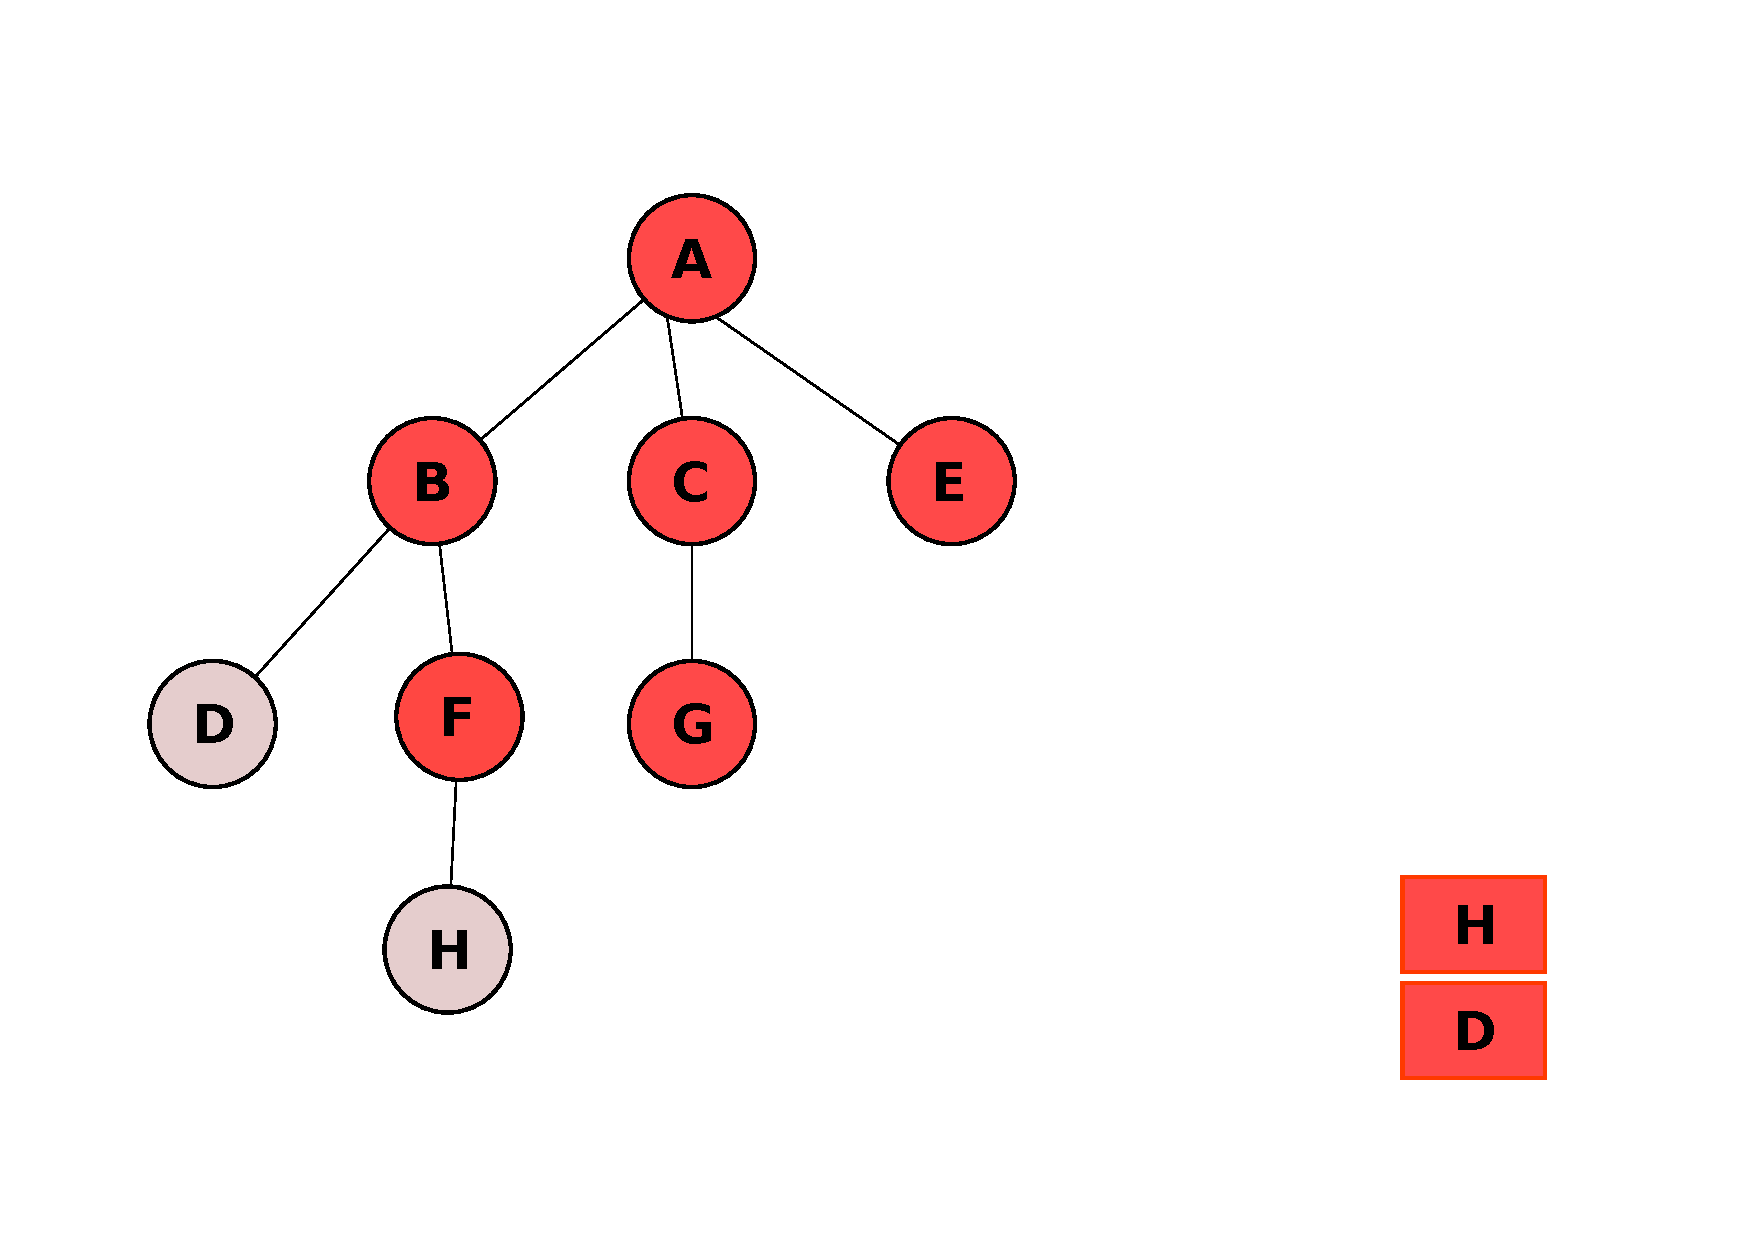
\includegraphics[scale=0.35]{figs/graph_dfs_HD}
\end{figure}
}
\only<9>{
\begin{figure}
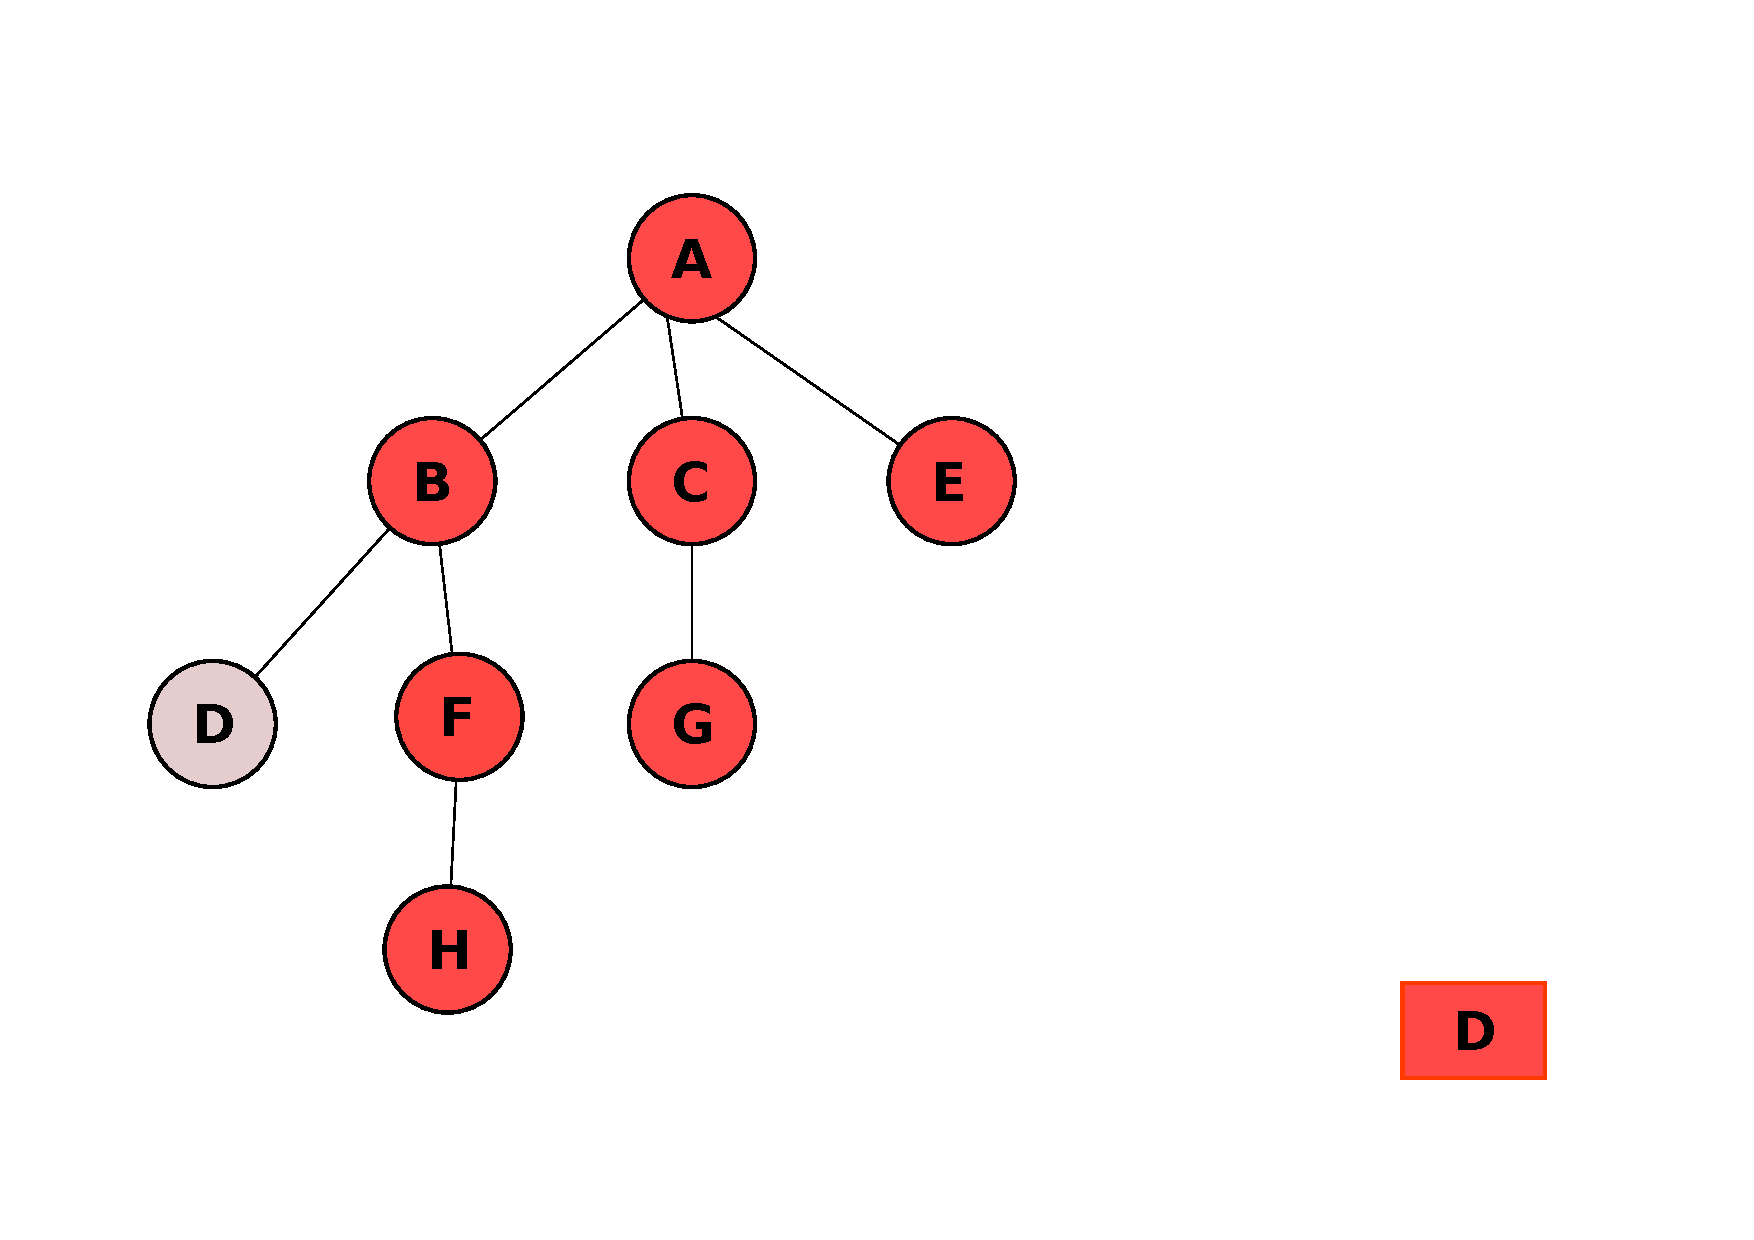
\includegraphics[scale=0.35]{figs/graph_dfs_D}
\end{figure}
}
\only<10>{
\begin{figure}
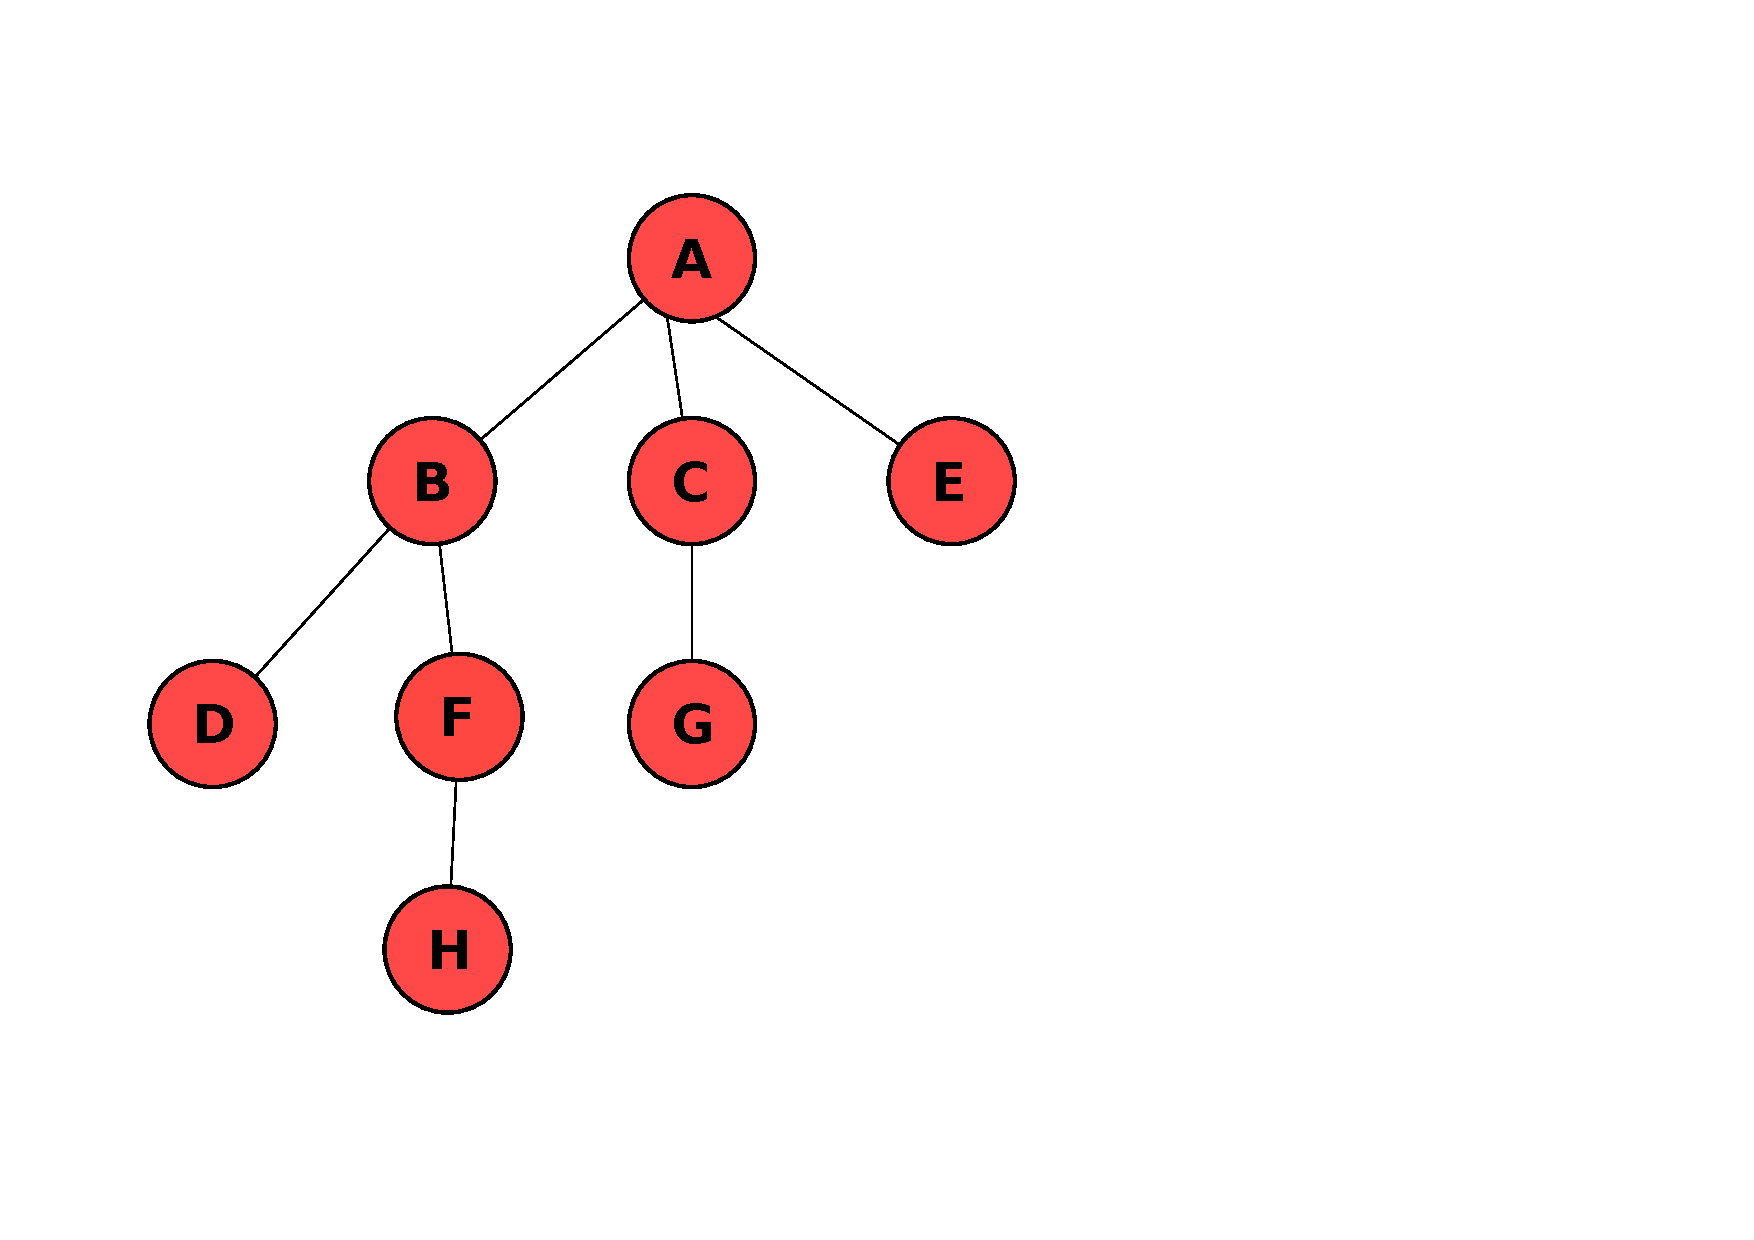
\includegraphics[scale=0.35]{figs/graph_dfs_full}
\end{figure}
}

\end{frame}

\begin{frame}{TDA Pile}{Implémentation}

\begin{itemize}
\item La pile est un type de donnée abstrait. 
\item Classiquement, elle peut être implémentée à partir d'un tableau
\item Mais aussi à partir d'une liste chaînée 
\item En \textcolor{blueemph}{Java}, on utilisera la classes \texttt{Stack} (synchronisée) ou l'interface \texttt{Deque}. 
\end{itemize}
\end{frame}


\begin{frame}{Exemple}{Inverser une chaîne de caractères}
\only<1>{
\begin{figure}
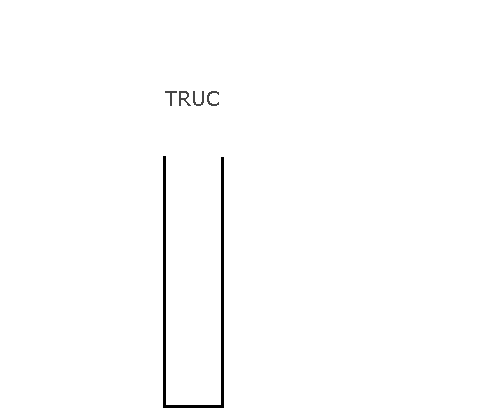
\includegraphics[scale=1]{figs/stack_word}
\end{figure}
}

\only<2>{
\begin{figure}
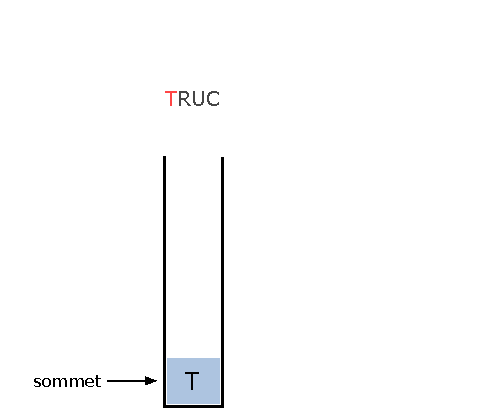
\includegraphics[scale=1]{figs/stack_t}
\end{figure}
}

\only<3>{
\begin{figure}
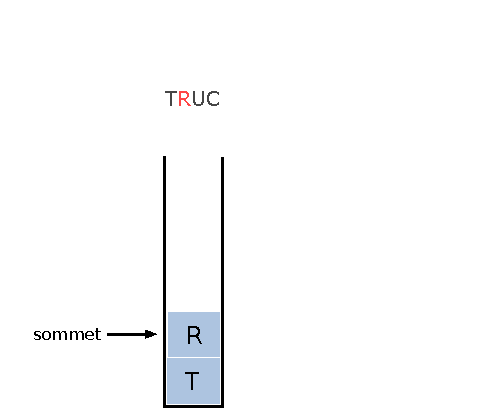
\includegraphics[scale=1]{figs/stack_tr}
\end{figure}
}

\only<4>{
\begin{figure}
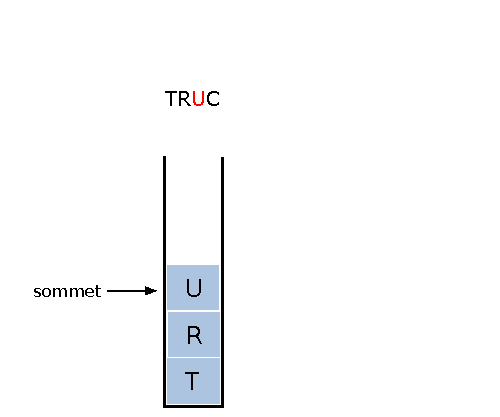
\includegraphics[scale=1]{figs/stack_tru}
\end{figure}
}

\only<5>{
\begin{figure}
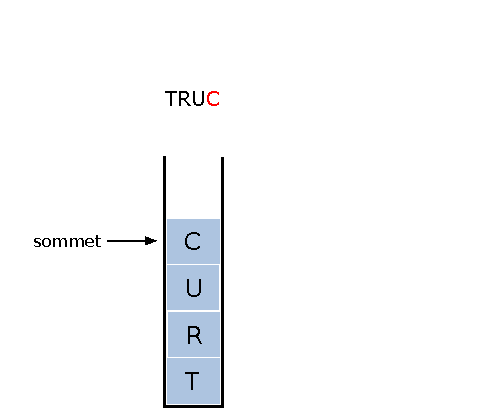
\includegraphics[scale=1]{figs/stack_truc}
\end{figure}
}

\only<6>{
\begin{figure}
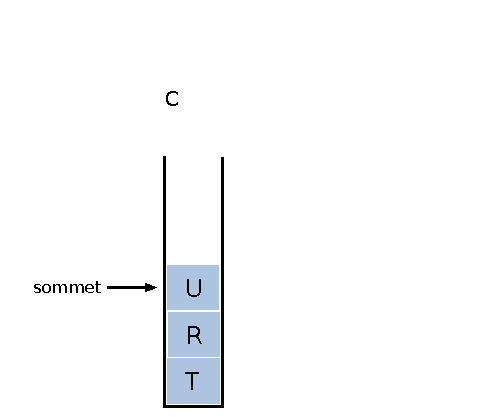
\includegraphics[scale=1]{figs/stack_c}
\end{figure}
}
\only<7>{
\begin{figure}
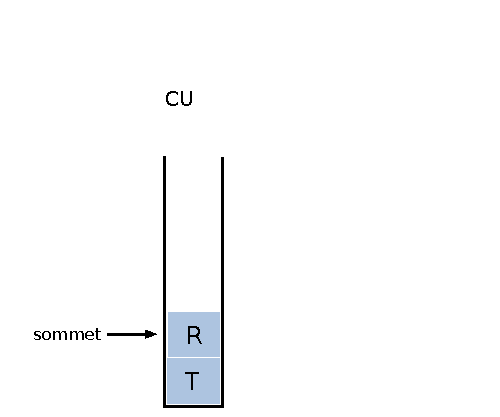
\includegraphics[scale=1]{figs/stack_cu}
\end{figure}
}
\only<8>{
\begin{figure}
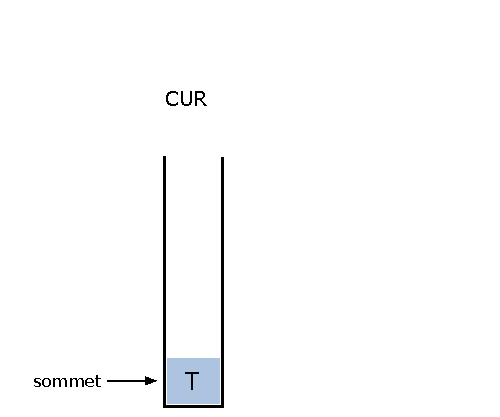
\includegraphics[scale=1]{figs/stack_cur}
\end{figure}
}
\only<9>{
\begin{figure}
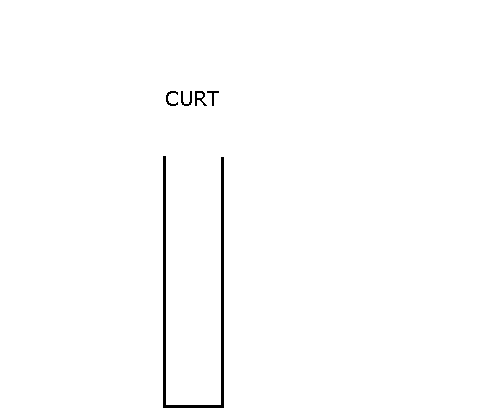
\includegraphics[scale=1]{figs/stack_curt}
\end{figure}
}

\end{frame}


\begin{frame}[fragile]{Code}{Inverser une chaîne de caractères}
\begin{lstlisting}
String input = "TRUC";
String output = "";

Stack <Character> stack = new Stack <Character>();

for(int i = 0; i < input.length(); i++){
  stack.push(input.charAt(i));
}
while(!stack.isEmpty()){
  output+=stack.pop();  
}

\end{lstlisting}

\end{frame}



\begin{frame}
\tableofcontents
\end{frame}

\section{Files}

\begin{frame}{Des files, pourquoi?}
Quelques exemples d'utilisation:
\begin{itemize}
\item File d'attente dans un magasin
\item Gestion de stocks de denrées périssables
\item Ordonnancement de processus
\end{itemize}
\end{frame}


\begin{frame}{File}{}
\begin{itemize}
\item Une file est un conteneur d'éléments qui respecte le principe du \textcolor{blueemph}{\textit{First In First Out}} (FIFO): le premier élément accessible est le premier ajouté.
\item Le premier élément enlevé est le plus ancien de la file
\item On insert (enfile) les éléments par la \textcolor{blueemph}{queue} et on les retire (défile) par la \textcolor{blueemph}{tête} comme dans une file d'attente:
\end{itemize}
\begin{figure}
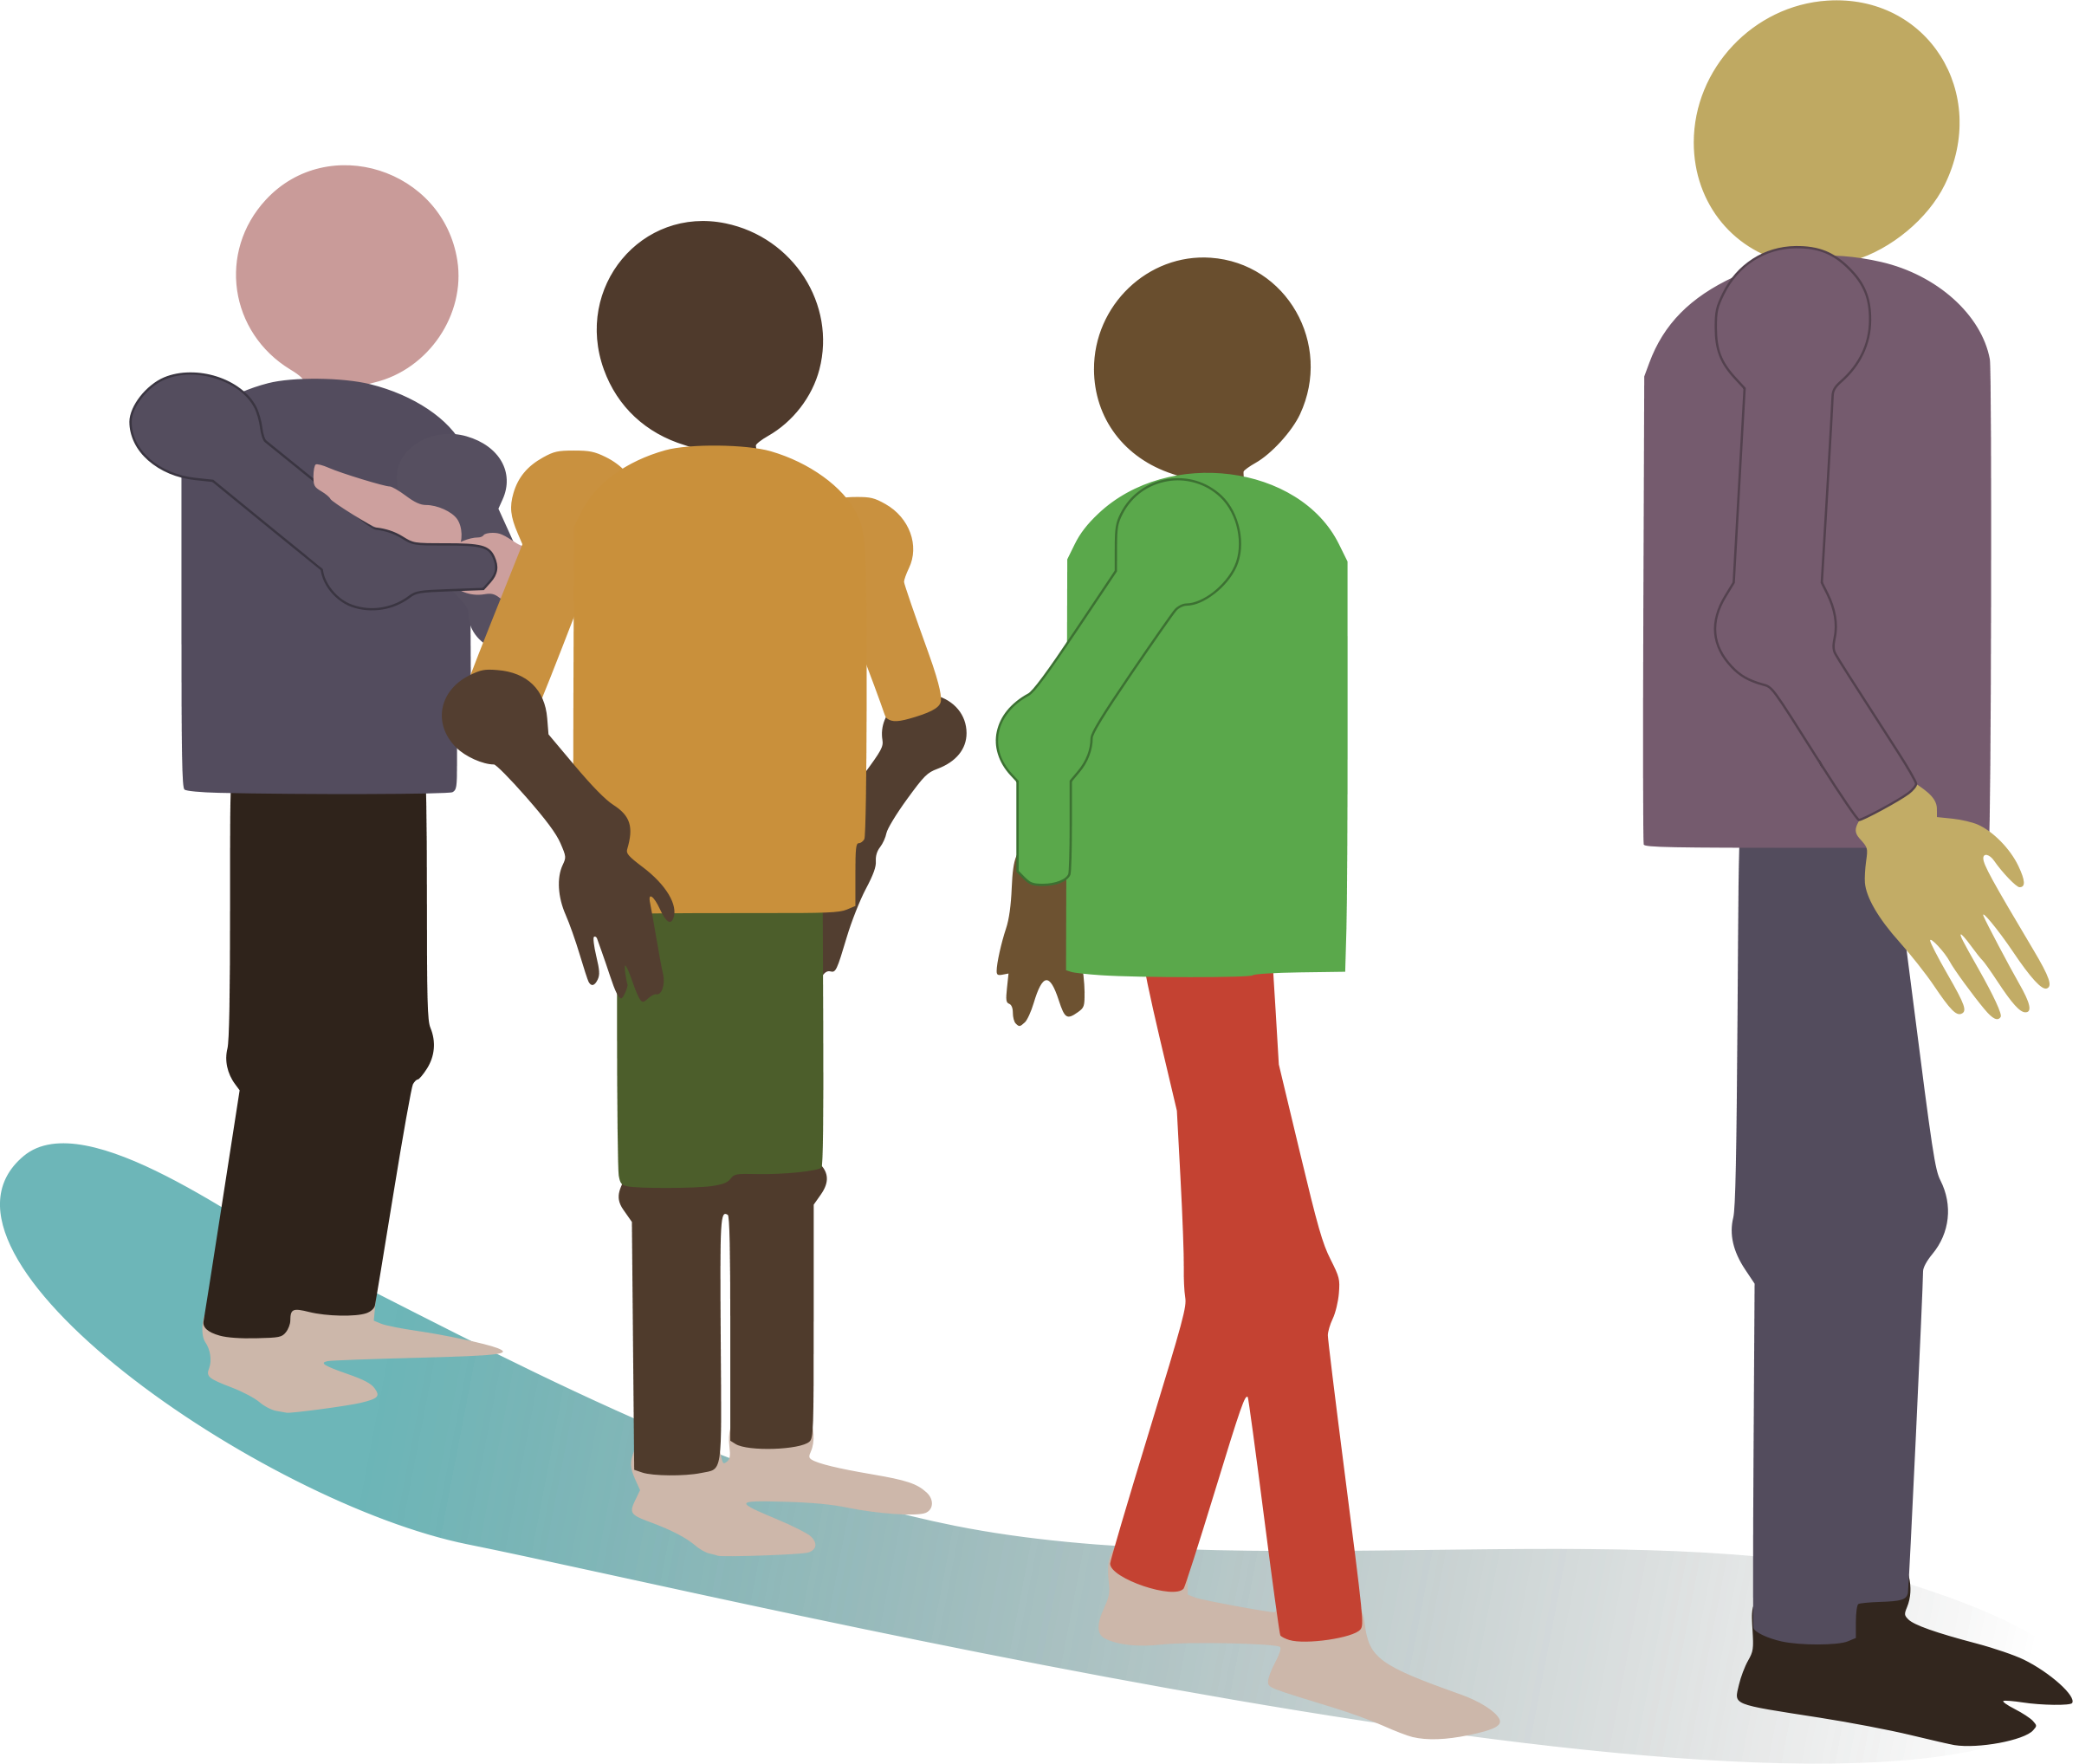
\includegraphics[scale=0.05]{figs/queue.png}
\end{figure}

\end{frame}


\begin{frame}{File: FIFO}
\only<1>{
File à l'origine:
\begin{figure}
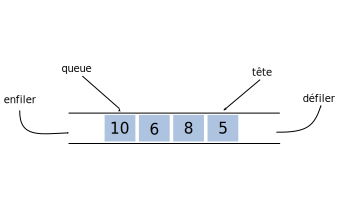
\includegraphics[scale=1]{figs/file}
\end{figure}
}

\only<2>{
On défile la valeur 5 en tête:
\begin{figure}
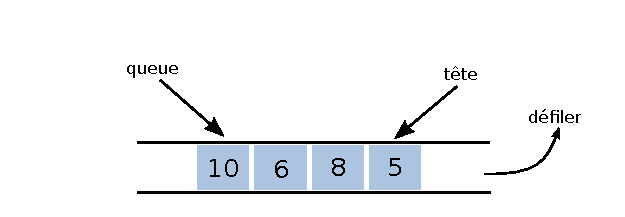
\includegraphics[scale=1]{figs/defiler}
\end{figure}
}

\only<3>{
8 devient la valeur en tête de ma file:
\begin{figure}
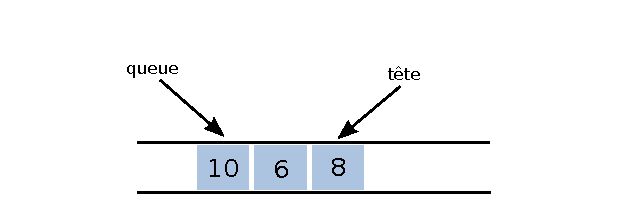
\includegraphics[scale=1]{figs/defiler2}
\end{figure}
}

\only<4>{
On enfile 14:
\begin{figure}
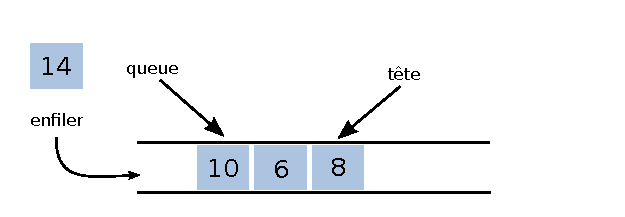
\includegraphics[scale=1]{figs/enfiler}
\end{figure}
}

\only<5>{
14 devient la valeur en queue de file:
\begin{figure}
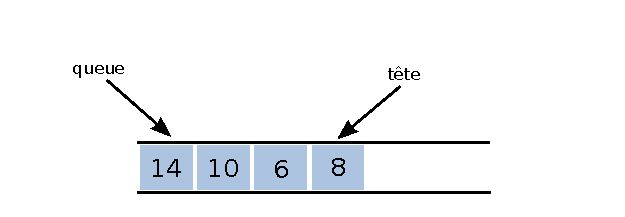
\includegraphics[scale=1]{figs/enfiler2}
\end{figure}
}


\end{frame}

\begin{frame}{TDA File}{Opérations}
Le type de données abstrait File spécifie plusieurs opérations principales :
\begin{itemize}
\item \texttt{enfile(T val)} : Ajoute une valeur val de type T en queue de file
\item \texttt{T défiler()} : Retire une valeur en tête
\item \texttt{T tête()}: Retourne (sans la retirer) la valeur en tête de file
\item \texttt{int taille()}: Retourne le nombre d'éléments
\item \texttt{boolean estVide()} : teste si la file est vide
\end{itemize}

\end{frame}

\begin{frame}{Application: \textcolor{blueemph}{Parcours en largeur}}
\only<1>{
\begin{figure}
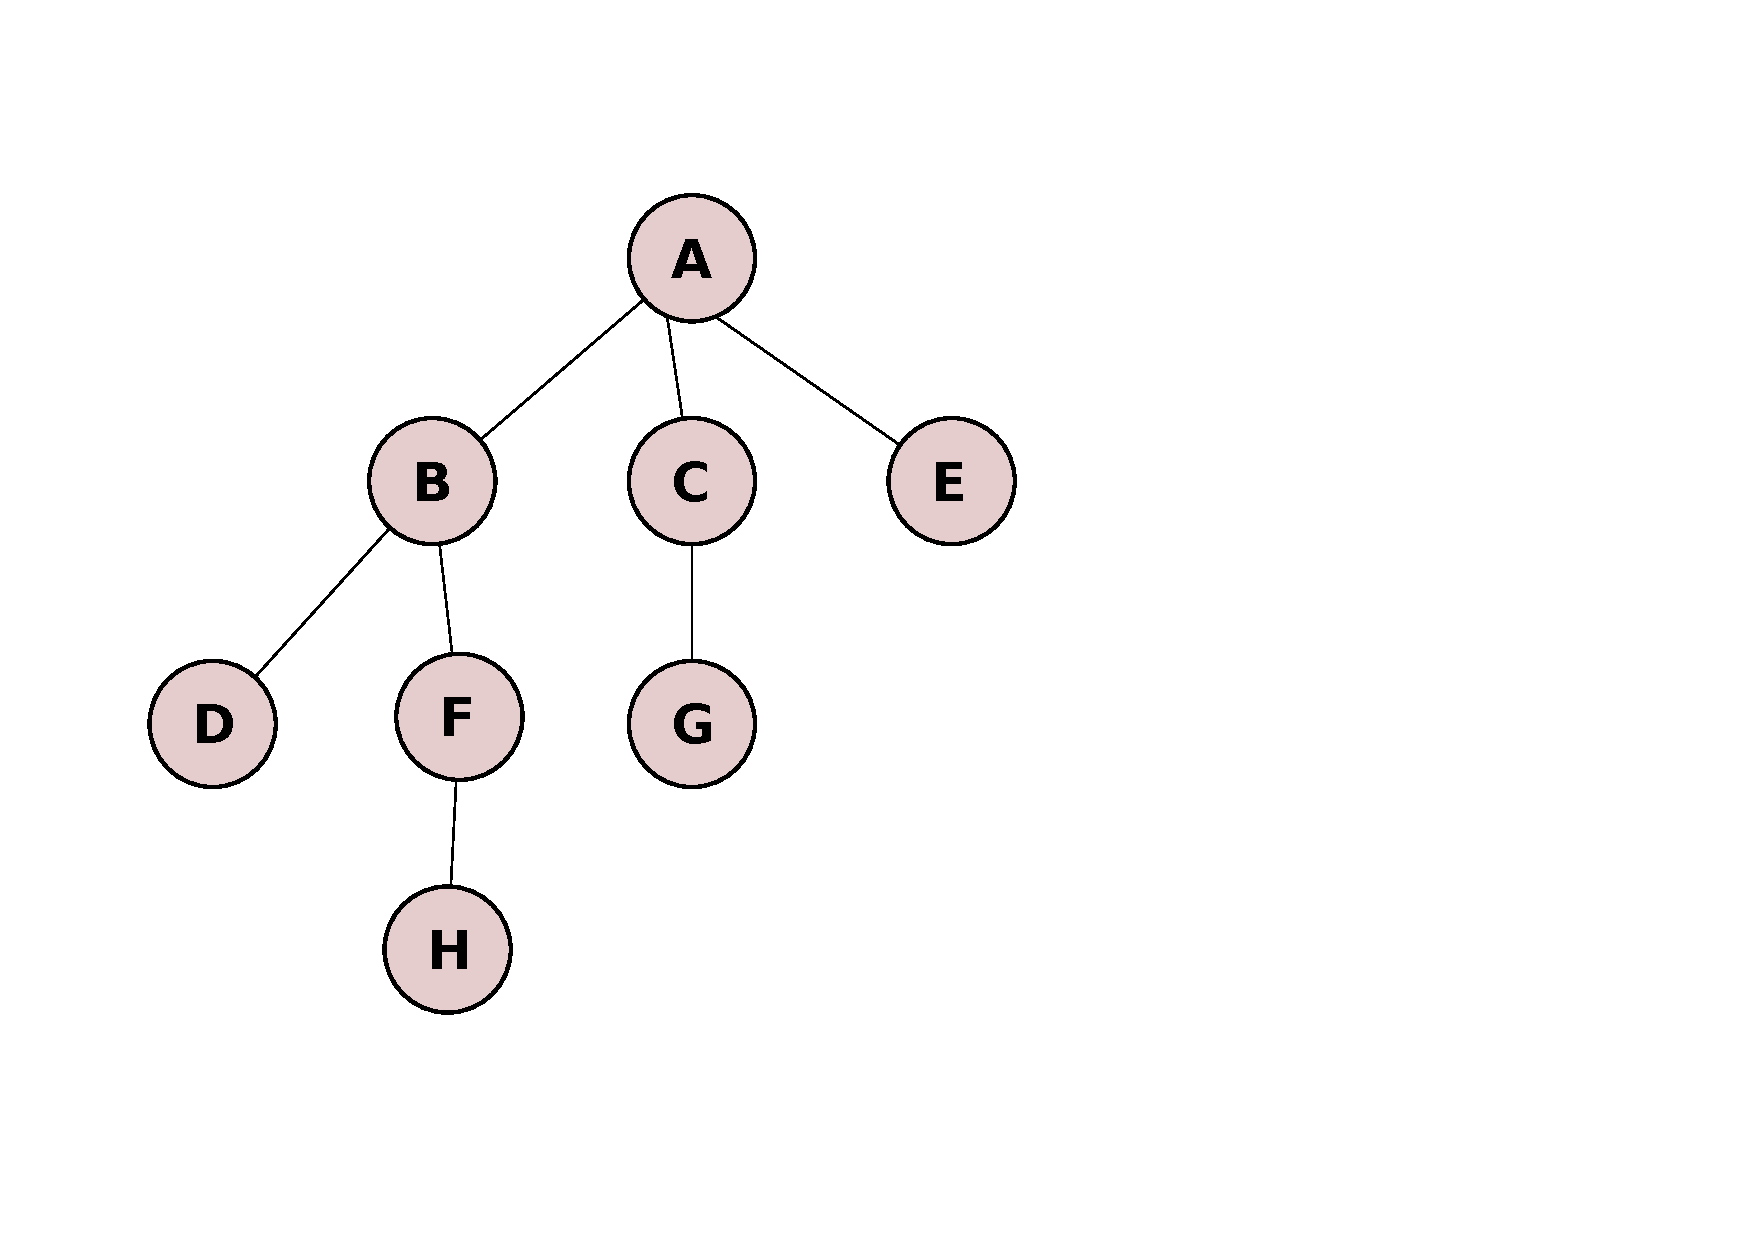
\includegraphics[scale=0.35]{figs/graph}
\end{figure}
}

\only<2>{
\begin{figure}
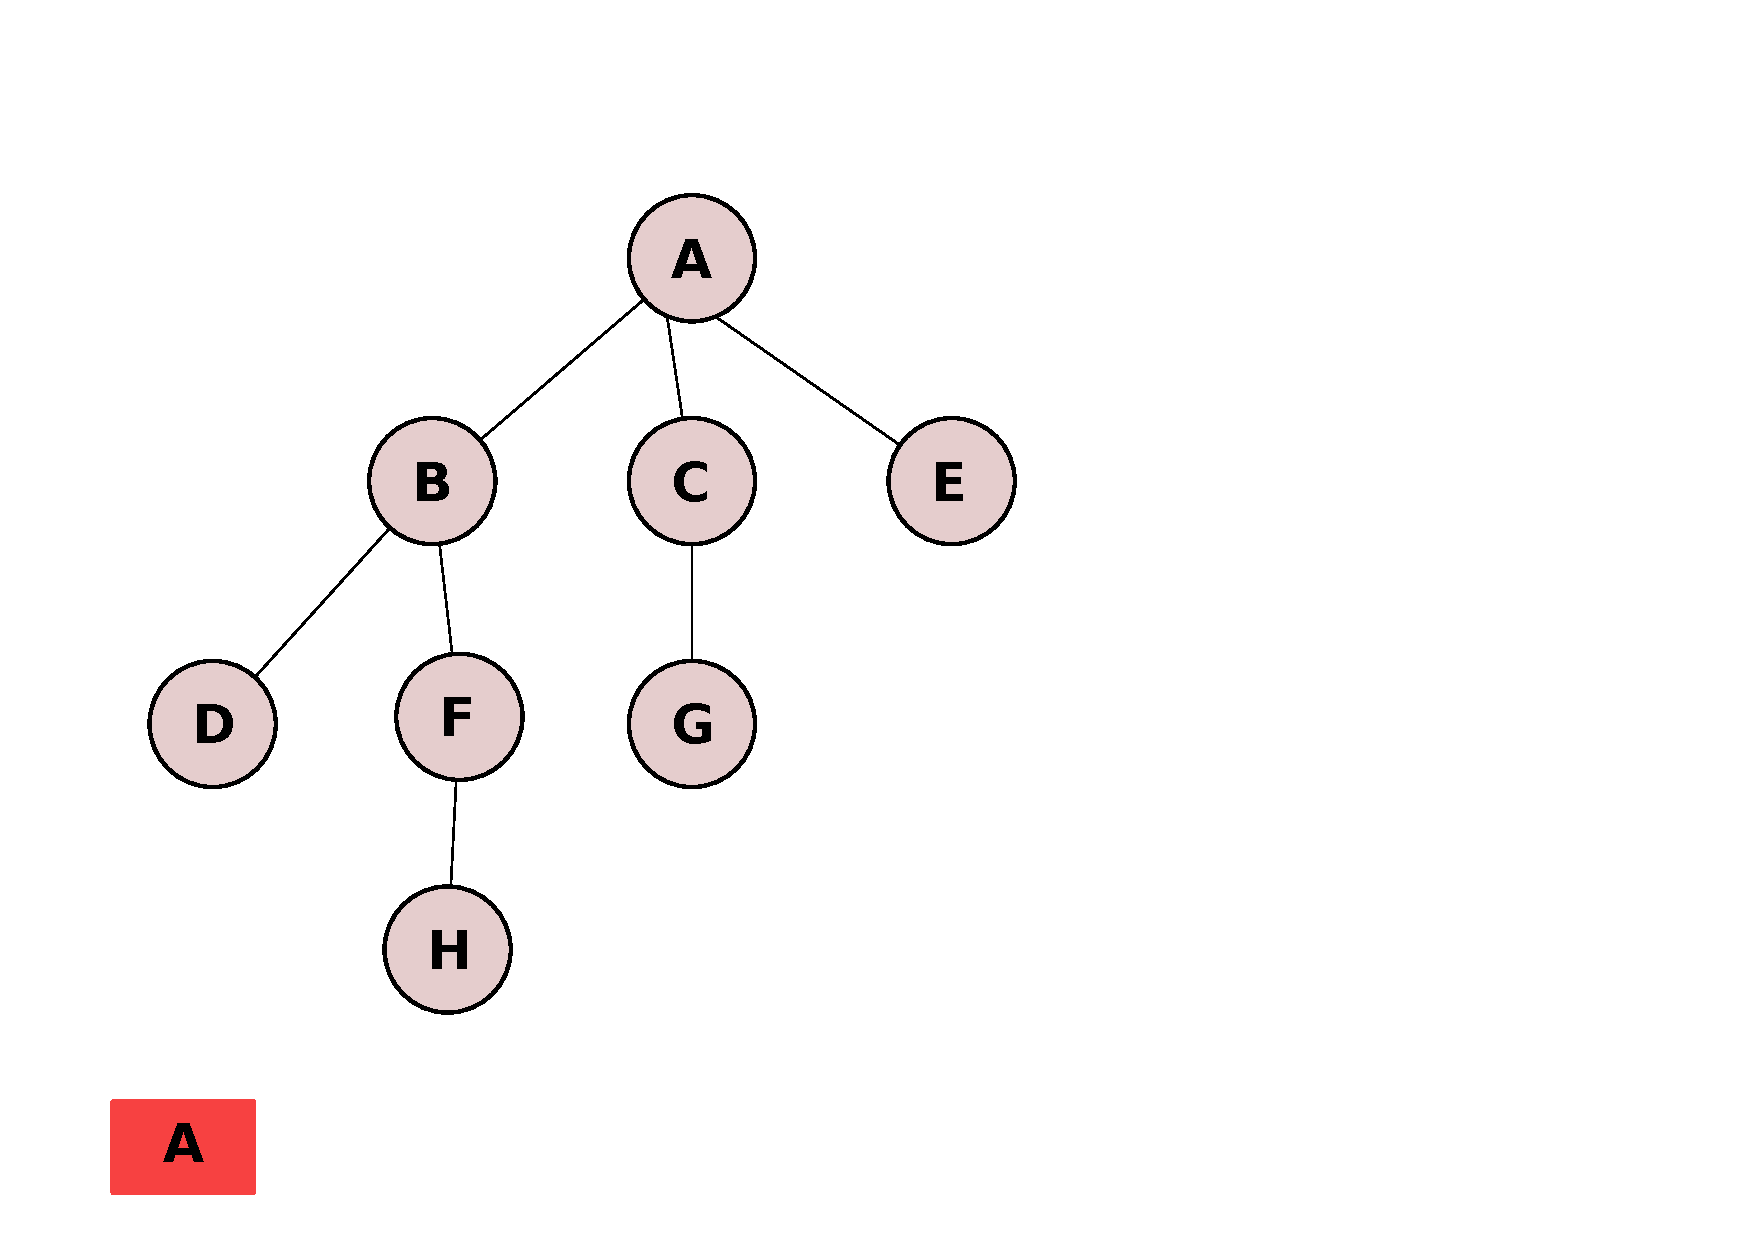
\includegraphics[scale=0.35]{figs/graph_bfs_A}
\end{figure}
}

\only<3>{
\begin{figure}
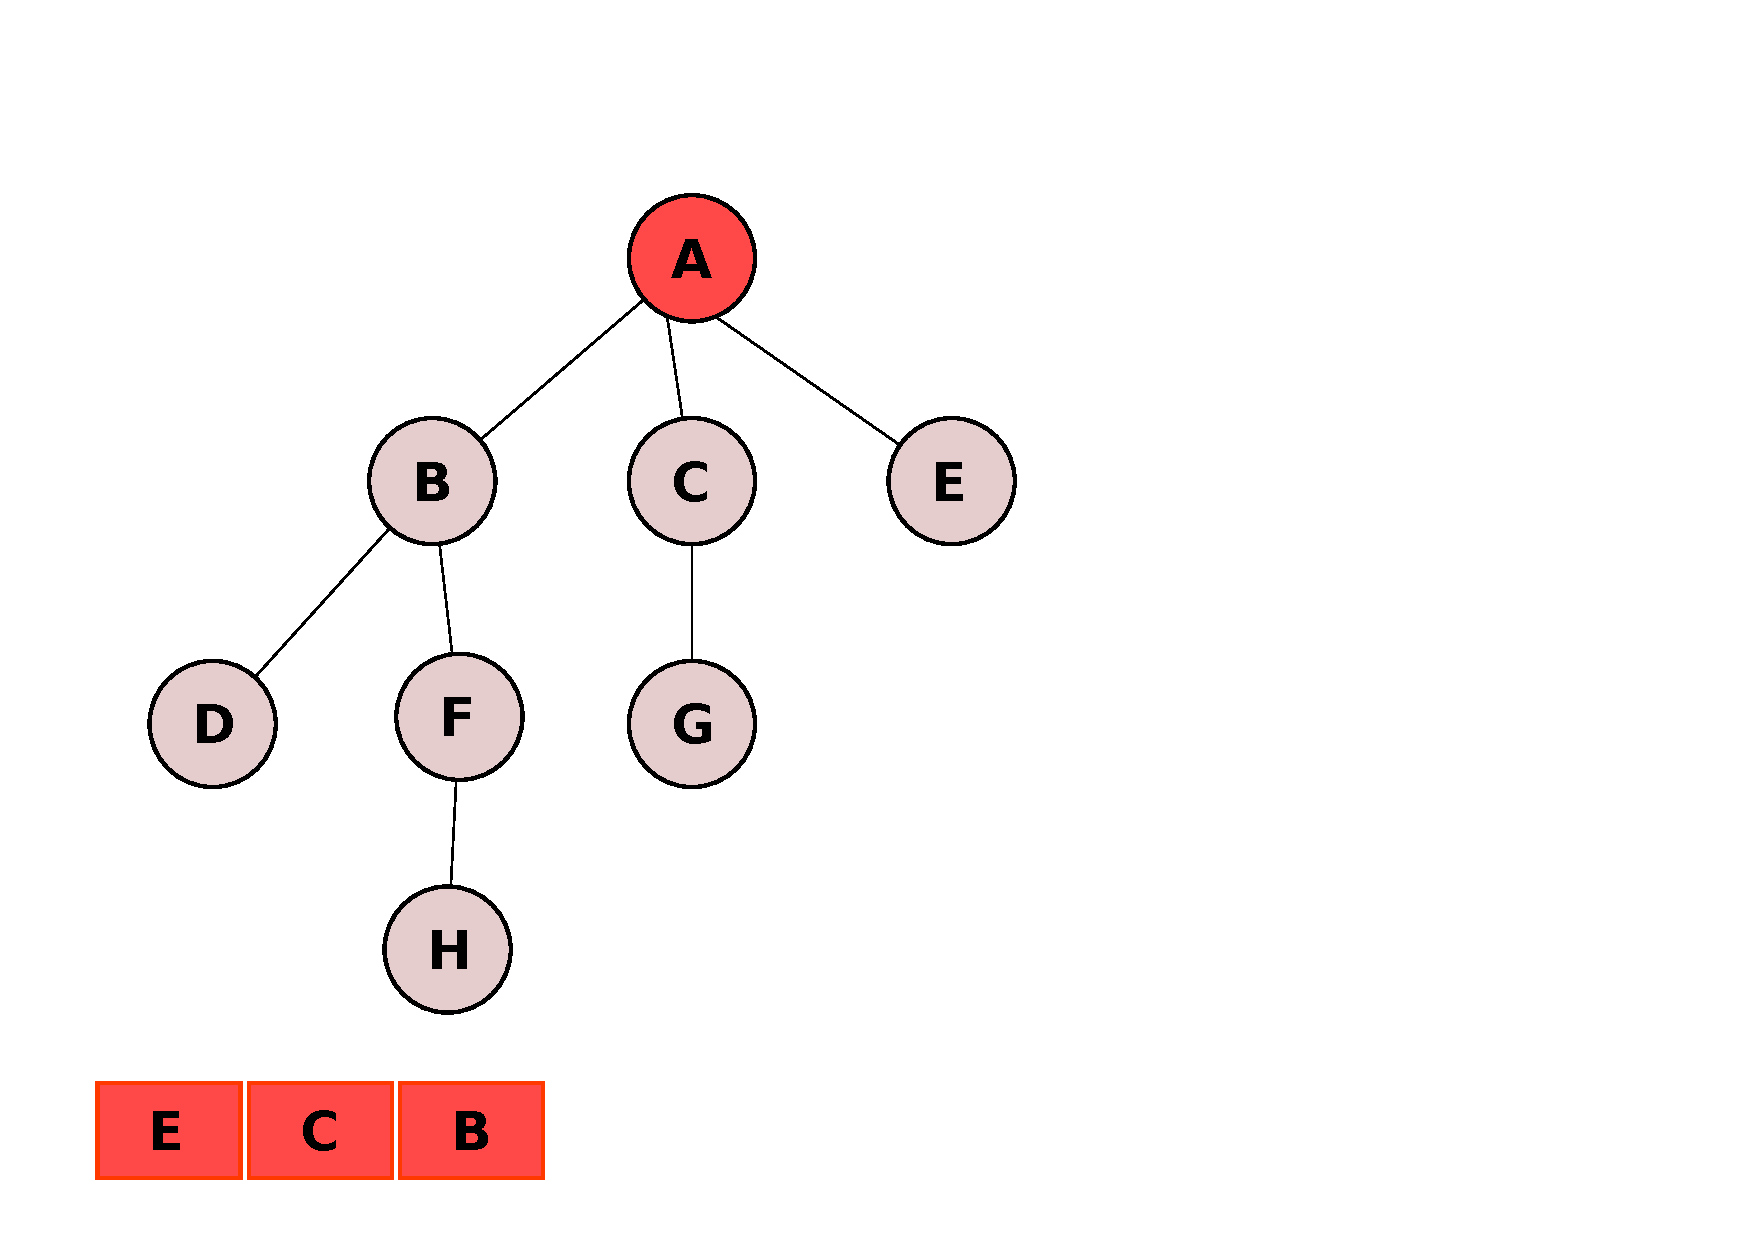
\includegraphics[scale=0.35]{figs/graph_bfs_ECB}
\end{figure}
}

\only<4>{
\begin{figure}
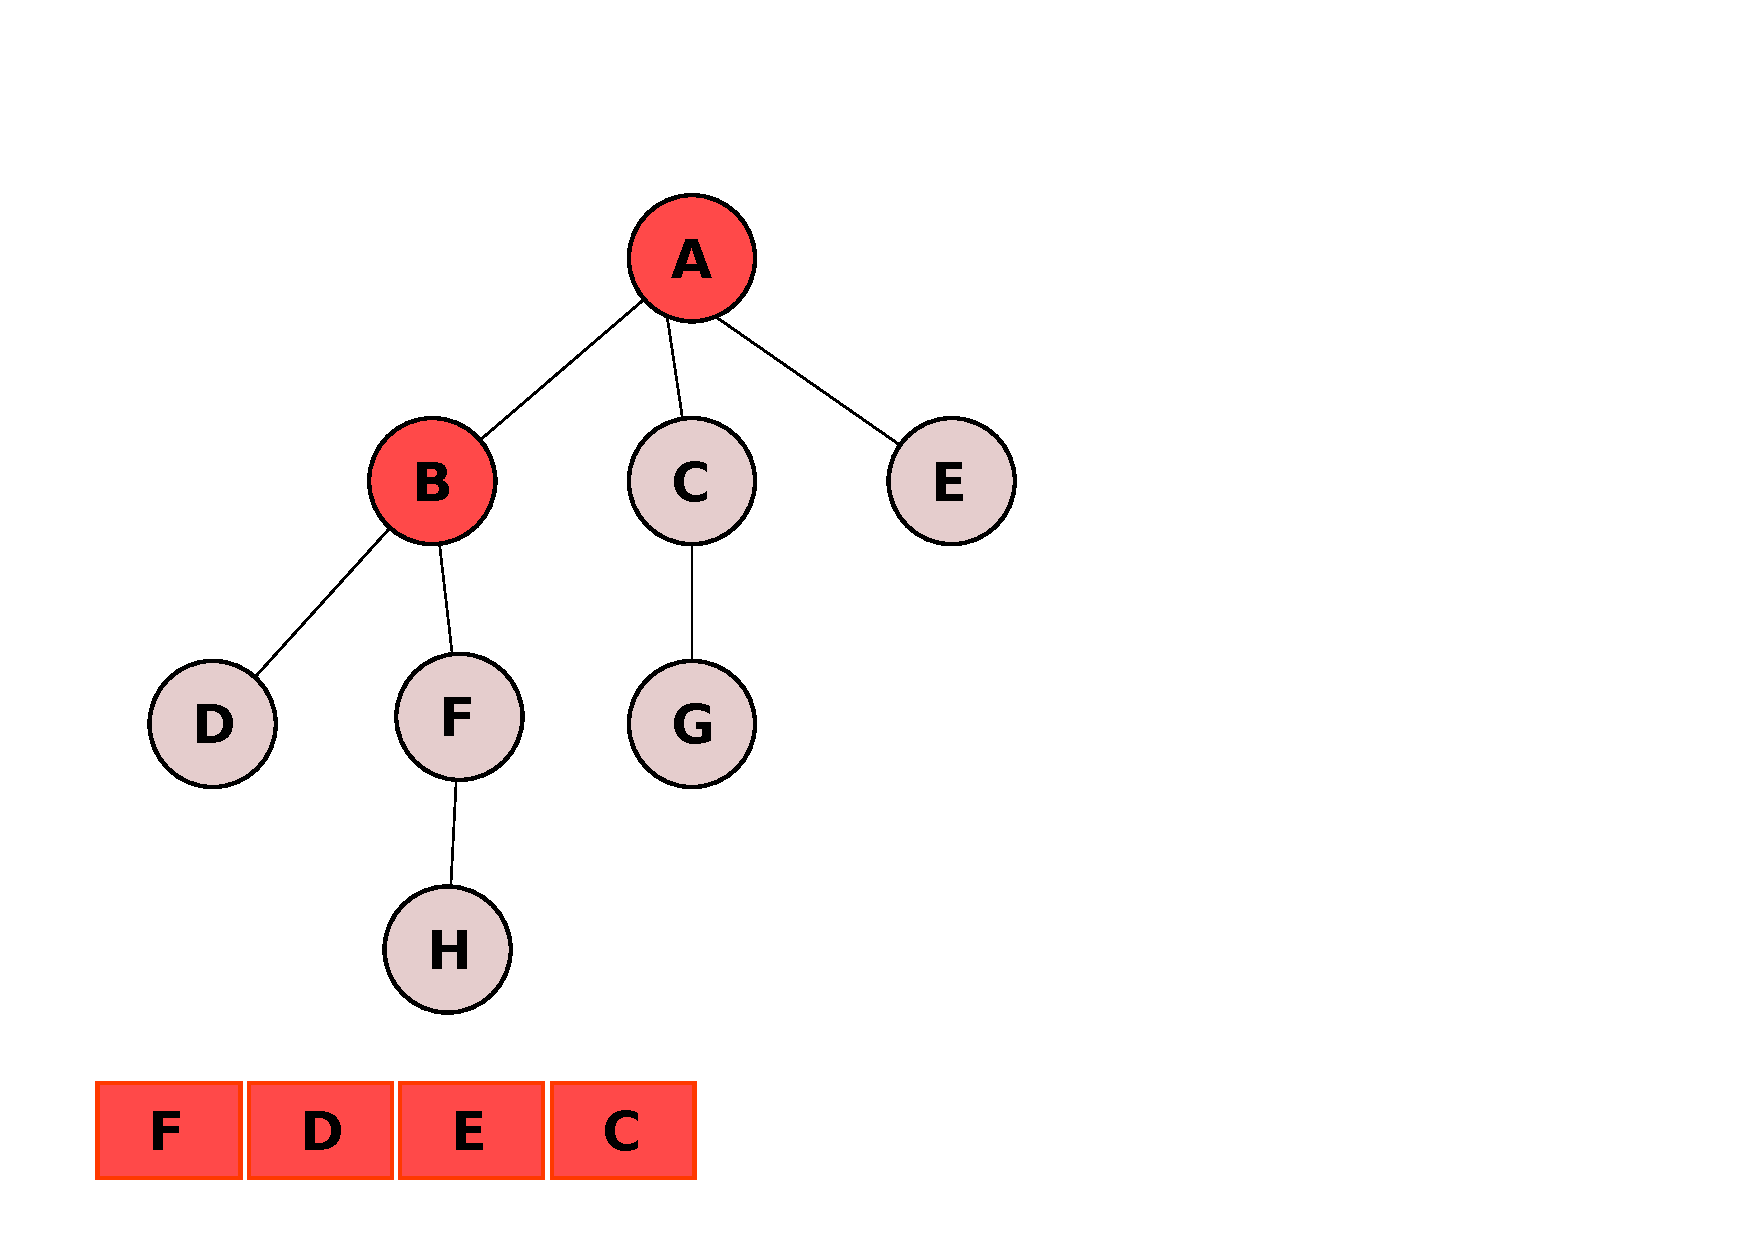
\includegraphics[scale=0.35]{figs/graph_bfs_FDEC}
\end{figure}
}

\only<5>{
\begin{figure}
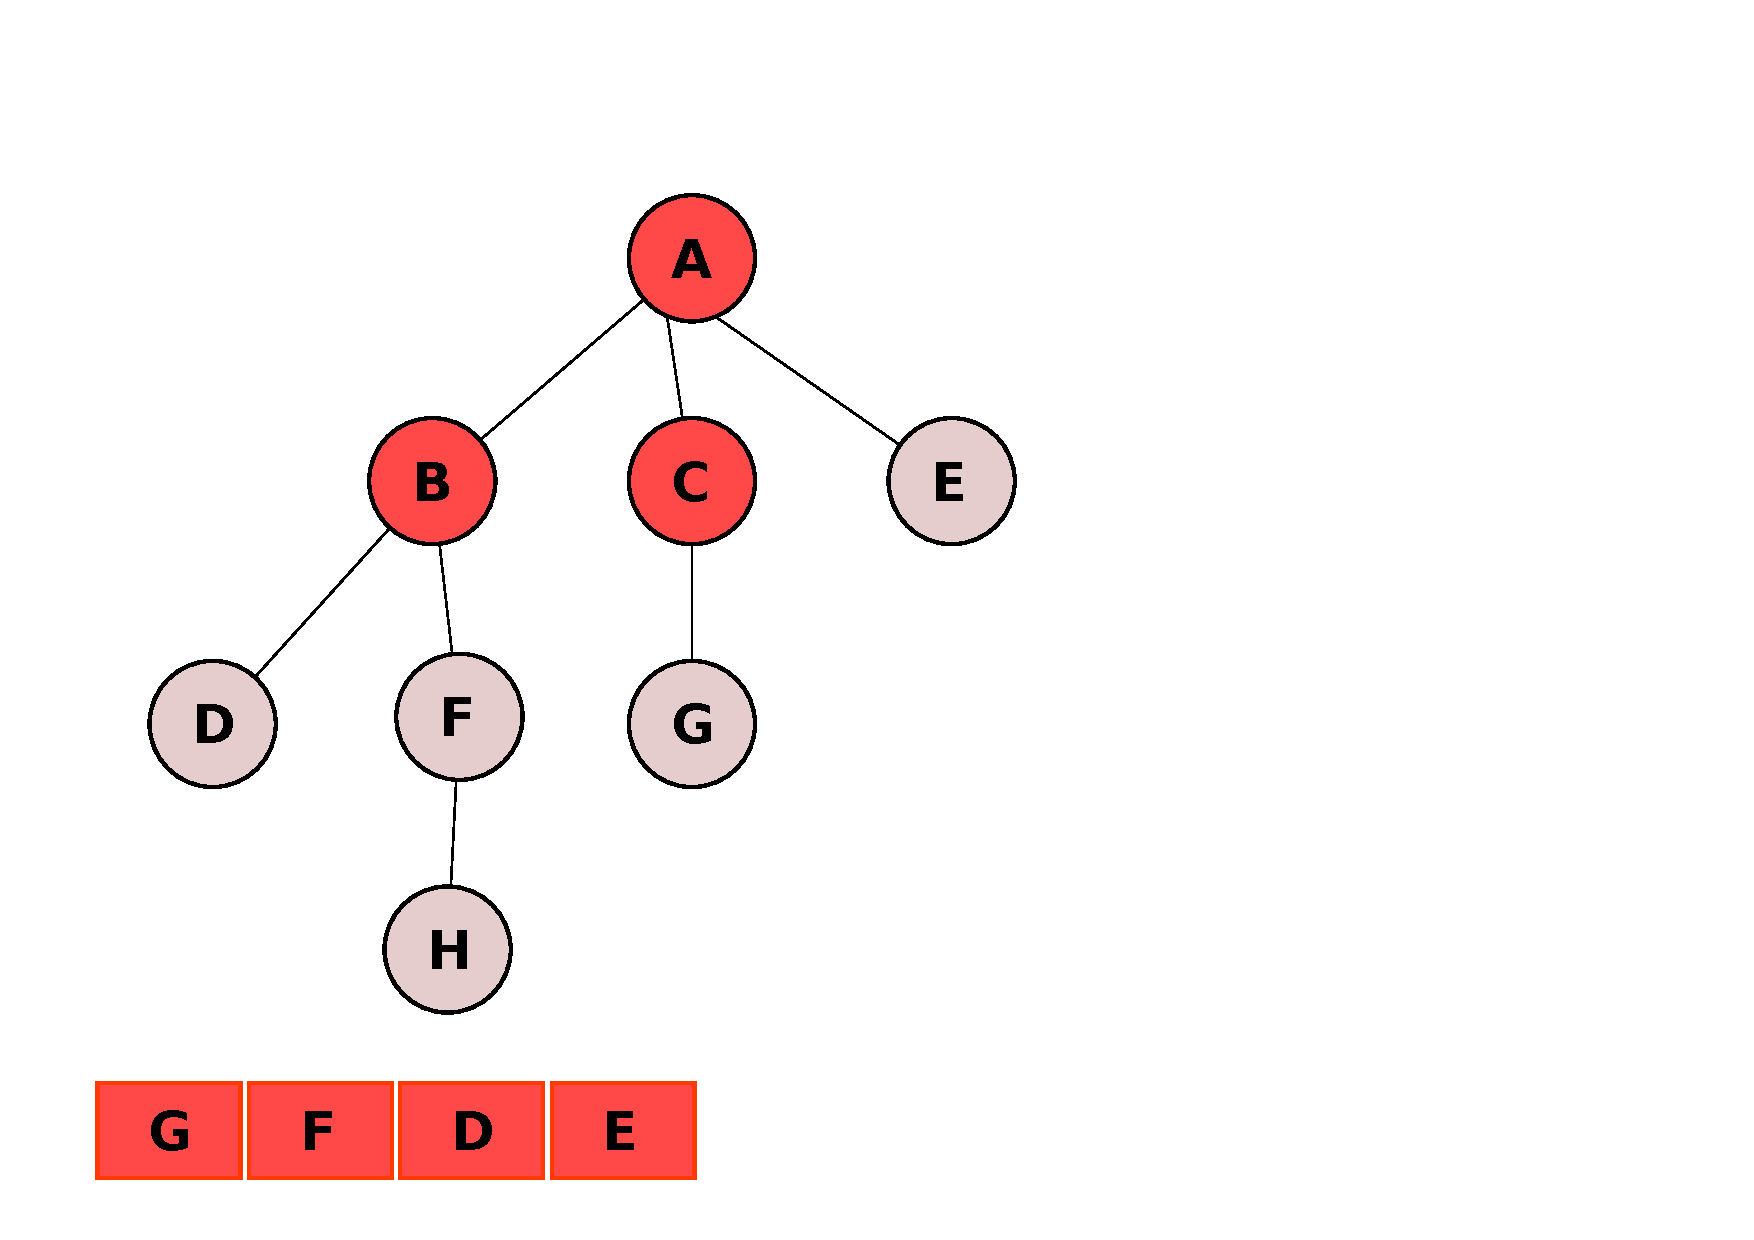
\includegraphics[scale=0.35]{figs/graph_bfs_GFDE}
\end{figure}
}

\only<6>{
\begin{figure}
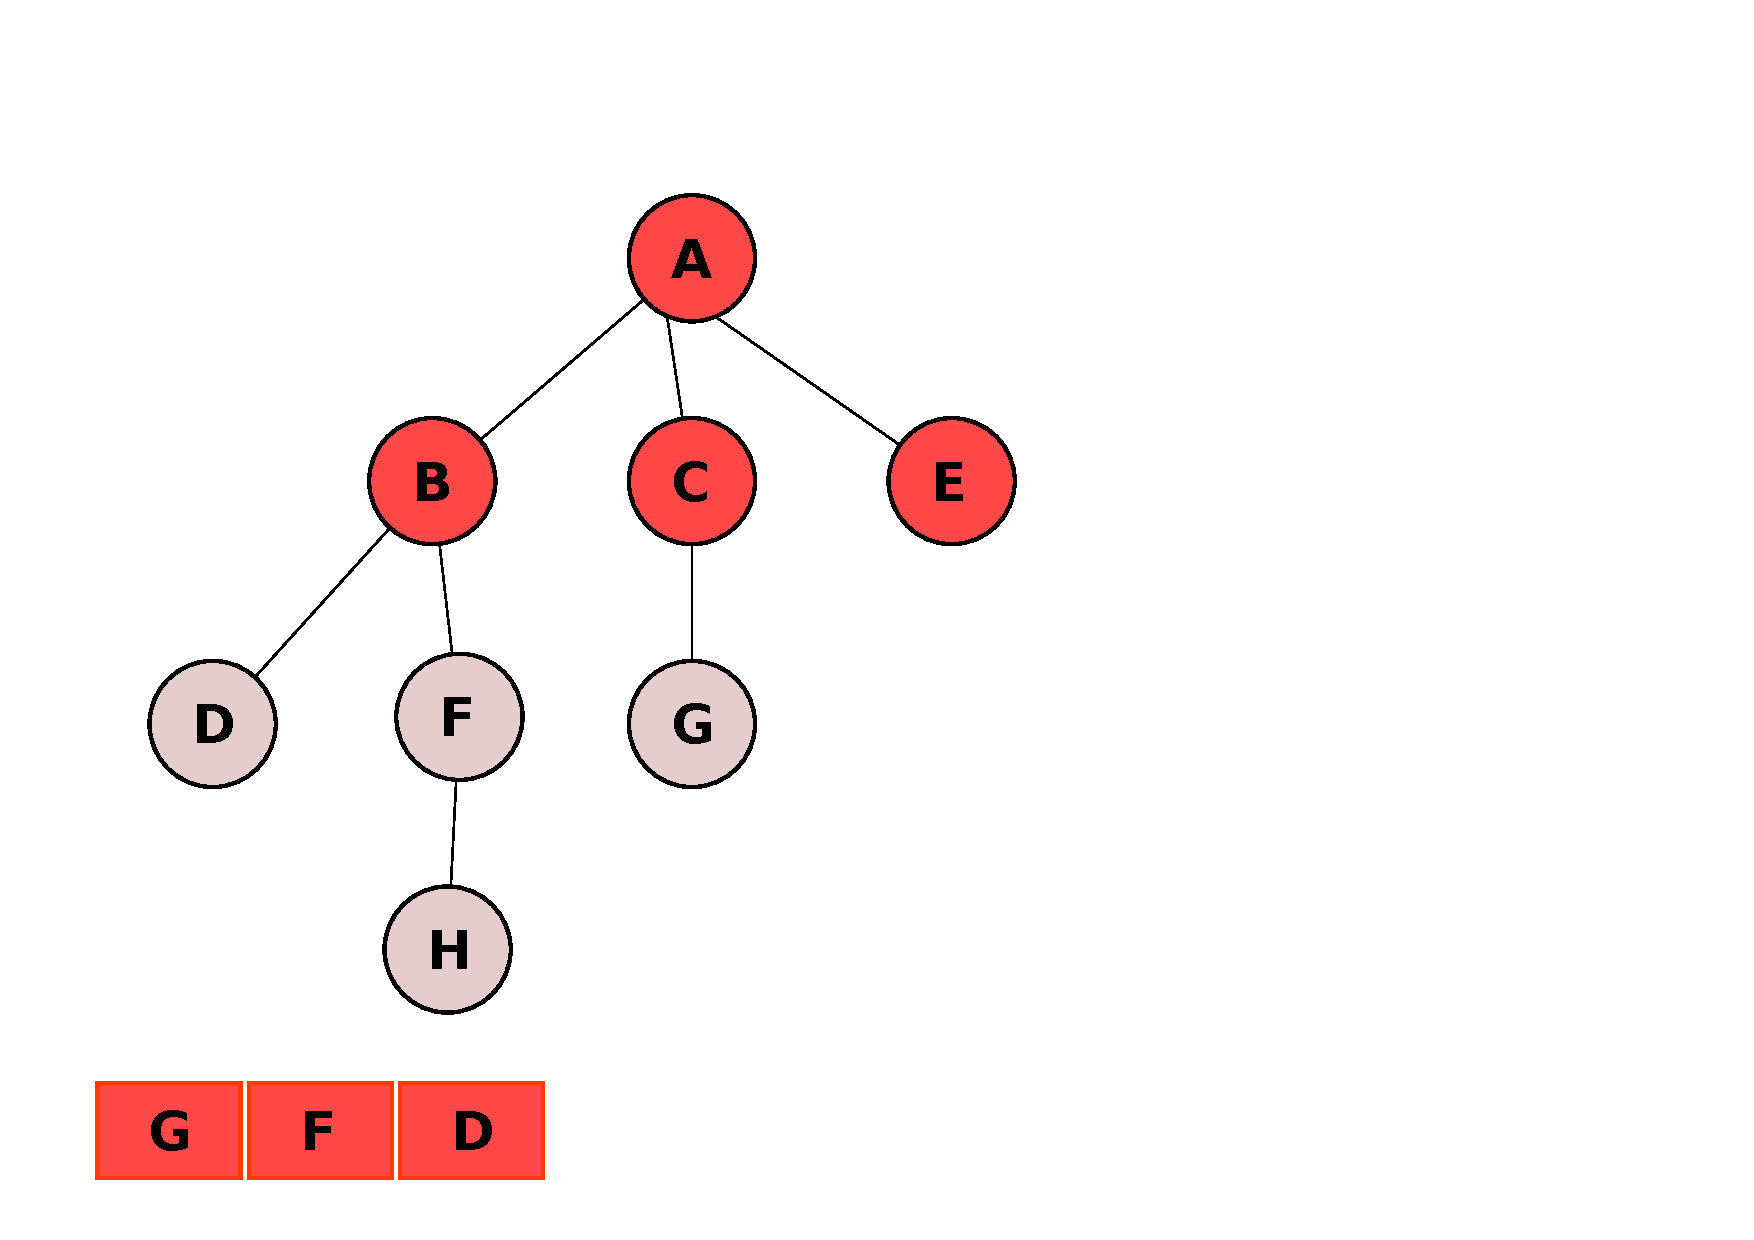
\includegraphics[scale=0.35]{figs/graph_bfs_GFD}
\end{figure}
}
\only<7>{
\begin{figure}
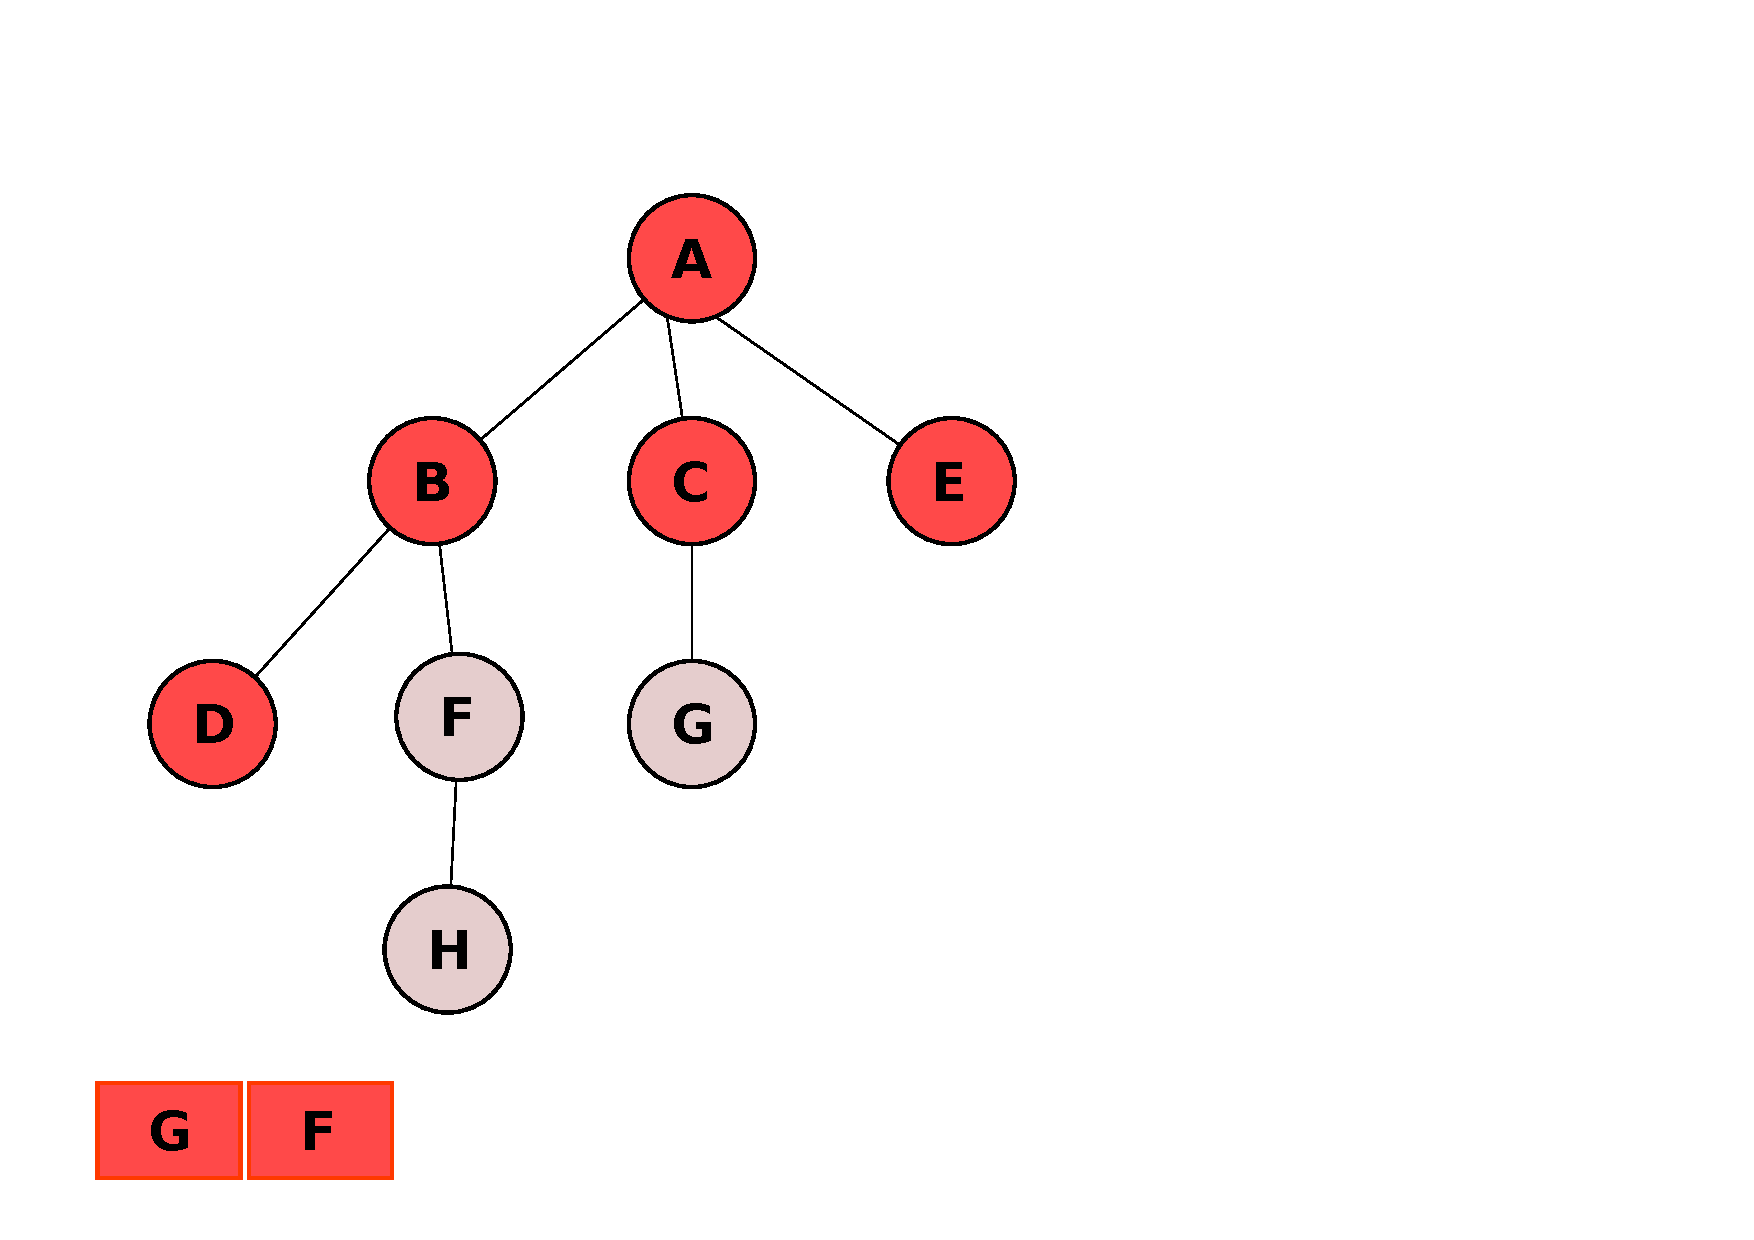
\includegraphics[scale=0.35]{figs/graph_bfs_GF}
\end{figure}
}
\only<8>{
\begin{figure}
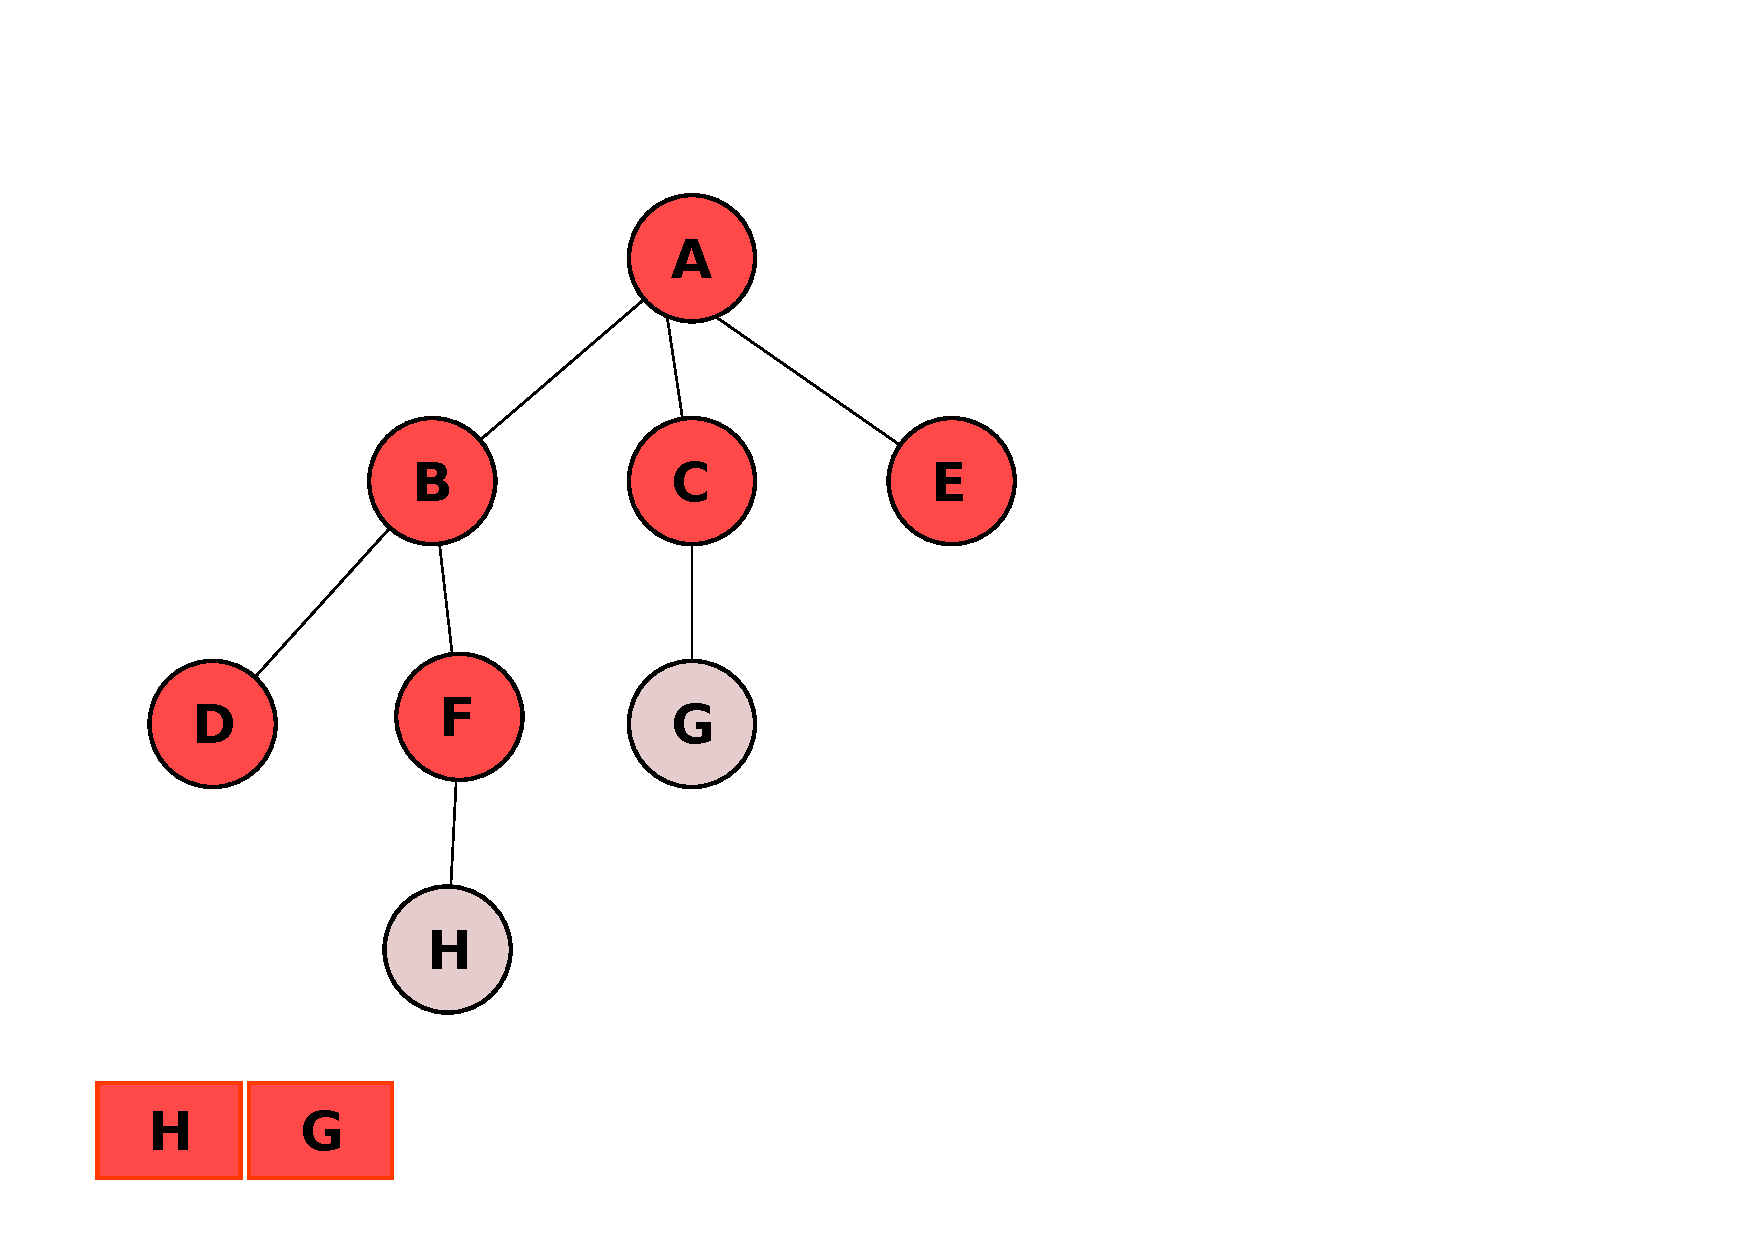
\includegraphics[scale=0.35]{figs/graph_bfs_HG}
\end{figure}
}
\only<9>{
\begin{figure}
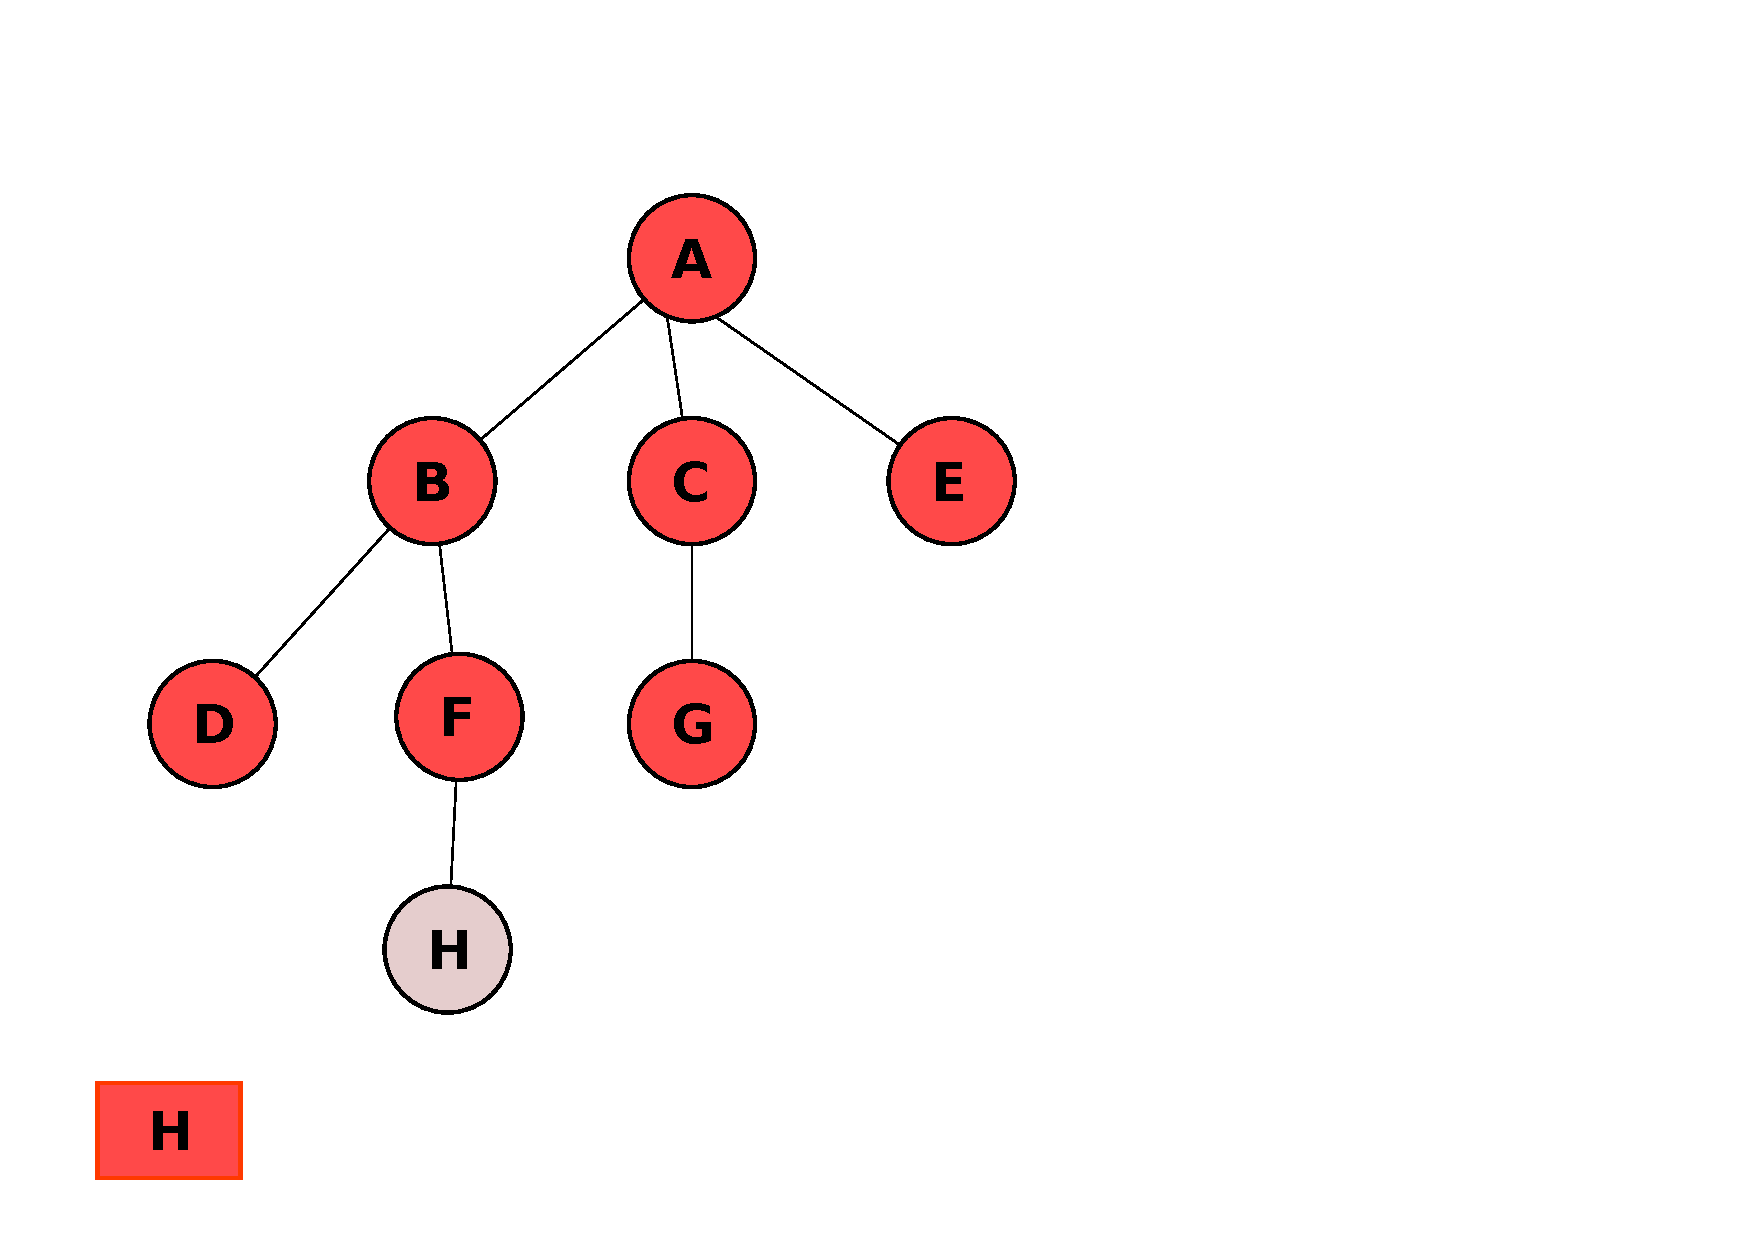
\includegraphics[scale=0.35]{figs/graph_bfs_H}
\end{figure}
}
\only<10>{
\begin{figure}
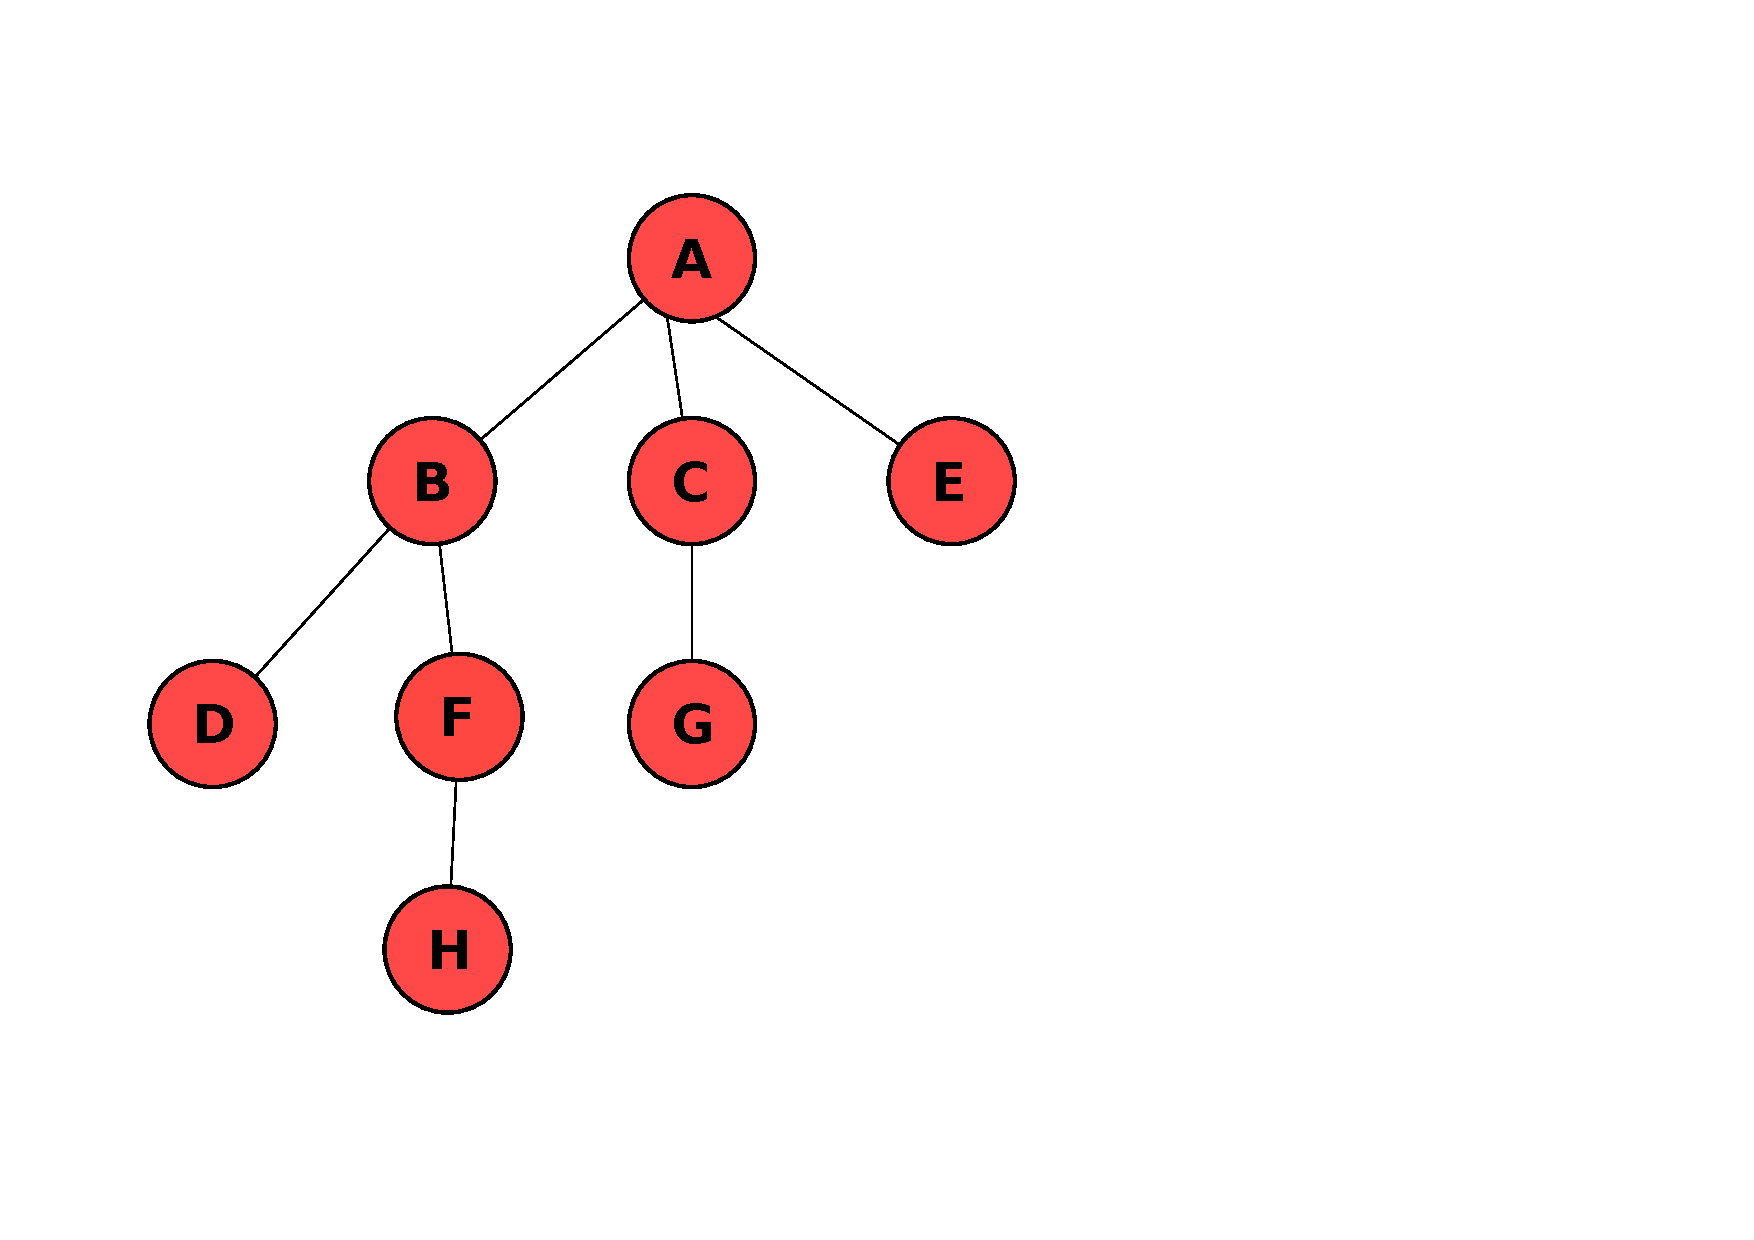
\includegraphics[scale=0.35]{figs/graph_dfs_full}
\end{figure}
}
\end{frame}


\begin{frame}{TDA File}{Implémentation}

\begin{itemize}
\item La file est un type de donnée abstrait
\item Elle pourrait être implémentée à partir d'un tableau
\item Mais le plus souvent, une liste est utilisée
\item En \textcolor{blueemph}{Java}, on utilisera l'interface $Queue$ ou $Deque$.
\end{itemize}


\end{frame}

\begin{frame}[fragile]
\begin{lstlisting}
public class MyQueue <T>{
    private LinkedList<T> list;

    public MyQueue(){
        list = new LinkedList<T>();
    }
    public void enqueue( T element) {//
        list.addFirst(element);
    }
    public T dequeue() {
        return list.removeLast();
    }   
  
         public static void main(String[] args){
         MyQueue <Integer> q = new MyQueue <Integer>();
         q.enqueue(24);
         q.enqueue(34);
         int i = q.dequeue(); // i = 24
     }
}
\end{lstlisting}

\end{frame}

\begin{frame}{Bilan}
Dans ce cours nous avons vu:
\begin{itemize}
\item Deux nouveaux types de données abstraits,
\item Avec un accès limité à un seul élément,
\item Les piles : le dernier élément ajouté $\Rightarrow$ premier sorti,
\item Les files : le premier élément ajouté $\Rightarrow$ premier sorti.
\end{itemize}
\end{frame}

\begin{frame}{Expressions arithmétiques}
 \begin{itemize}
 \item Notation infixée : 2 + 5
 \item Notation postfixée : 2 5 +
 \item Notation préfixée : + 2 5 
 \end{itemize}

\end{frame}

\begin{frame}{Expressions arithmétiques}
70 + 150 * 1.0725 =  235.95 ou 230.875 ?
\newline
\pause
Notation postfixée: 70  150 + 1.0725 *\newline
\pause Les parenthèses ne sont nécessaires.

\end{frame}





\begin{frame}{Conversion infixée vers postfixée}{Principe}

\begin{itemize}
\item Quand un opérande est lu, on l'ajoute à la sortie
\item Quand un opérateur est lu, on l'empile si la pile est vide. Sinon, on dépile tous les opérateurs de priorité égale ou supérieure que l'on ajoute à la sortie et après on empile l'opérateur courant.
\item Quand une parenthèse ouvrante est lue, on l'empile
\item Quand une parenthèse fermante est lue, on dépile jusqu'à dépiler l'ouvrante et on ajoute les opérateurs à la sortie.
\item Quand on a fini de lire l'entrée, on dépile tous les éléments restants qu'on ajoute à la sortie.
\end{itemize}
\end{frame}

\begin{frame}{Conversion infixée vers postfixée}{Exemple}
\begin{itemize}
\item entrée : (3+7)*(6-5)/((4-2)*(2+3))
\item pile : 
\item sortie : 
\end{itemize}
\end{frame}

\begin{frame}{Conversion infixée vers postfixée}
\begin{itemize}
\item entrée : \textbf{(}3+7)*(6-5)/((4-2)*(2+3))
\item pile : (
\item sortie : 
\end{itemize}
\end{frame}

\begin{frame}{Conversion infixée vers postfixée}
\begin{itemize}
\item entrée : (\textbf{3}+7)*(6-5)/((4-2)*(2+3))
\item pile : (
\item sortie : 3
\end{itemize}
\end{frame}

\begin{frame}{Conversion infixée vers postfixée}
\begin{itemize}
\item entrée : (3\textbf{+}7)*(6-5)/((4-2)*(2+3))
\item pile : ( + 
\item sortie : 3
\end{itemize}
\end{frame}

\begin{frame}{Conversion infixée vers postfixée}
\begin{itemize}
\item entrée : (3+\textbf{7})*(6-5)/((4-2)*(2+3))
\item pile : ( + 
\item sortie : 3 7 
\end{itemize}
\end{frame}

\begin{frame}{Conversion infixée vers postfixée}
\begin{itemize}
\item entrée : (3+7\textbf{)}*(6-5)/((4-2)*(2+3))
\item pile :  
\item sortie : 3 7 +
\end{itemize}
\end{frame}

\begin{frame}{Conversion infixée vers postfixée}
\begin{itemize}
\item entrée : (3+7)\textbf{*}(6-5)/((4-2)*(2+3))
\item pile : *
\item sortie : 3 7 +
\end{itemize}
\end{frame}

\begin{frame}{Conversion infixée vers postfixée}
\begin{itemize}
\item entrée : (3+7)*\textbf{(}6-5)/((4-2)*(2+3))
\item pile : * (
\item sortie : 3 7 +
\end{itemize}
\end{frame}

\begin{frame}{Conversion infixée vers postfixée}
\begin{itemize}
\item entrée : (3+7)*(\textbf{6}-5)/((4-2)*(2+3))
\item pile : * (
\item sortie : 3 7 + 6
\end{itemize}
\end{frame}

\begin{frame}{Conversion infixée vers postfixée}
\begin{itemize}
\item entrée : (3+7)*(6\textbf{-}5)/((4-2)*(2+3))
\item pile : * ( -
\item sortie : 3 7 + 6
\end{itemize}
\end{frame}

\begin{frame}{Conversion infixée vers postfixée}
\begin{itemize}
\item entrée : (3+7)*(6-\textbf{5})/((4-2)*(2+3))
\item pile : * ( -
\item sortie : 3 7 + 6 5 
\end{itemize}
\end{frame}

\begin{frame}{Conversion infixée vers postfixée}
\begin{itemize}
\item entrée : (3+7)*(6-\textbf{5})/((4-2)*(2+3))
\item pile : * ( -
\item sortie : 3 7 + 6 5 
\end{itemize}
\end{frame}
\begin{frame}{Conversion infixée vers postfixée}
\begin{itemize}
\item entrée : (3+7)*(6-5\textbf{)}/((4-2)*(2+3))
\item pile : *
\item sortie : 3 7 + 6 5 -
\end{itemize}
\end{frame}

\begin{frame}{Conversion infixée vers postfixée}
\begin{itemize}
\item entrée : (3+7)*(6-5)\textbf{/}((4-2)*(2+3))
\item pile : 
\item sortie : 3 7 + 6 5 - *
\end{itemize}
\end{frame}

\begin{frame}{Conversion infixée vers postfixée}
\begin{itemize}
\item entrée : (3+7)*(6-5)\textbf{/}((4-2)*(2+3))
\item pile : /
\item sortie : 3 7 + 6 5 - *
\end{itemize}
\end{frame}

\begin{frame}{Conversion infixée vers postfixée}
\begin{itemize}
\item entrée : (3+7)*(6-5)/\textbf{(}(4-2)*(2+3))
\item pile : / (
\item sortie : 3 7 + 6 5 - *
\end{itemize}
\end{frame}

\begin{frame}{Conversion infixée vers postfixée}
\begin{itemize}
\item entrée : (3+7)*(6-5)/(\textbf{(}4-2)*(2+3))
\item pile : / ( (
\item sortie : 3 7 + 6 5 - *
\end{itemize}
\end{frame}

\begin{frame}{Conversion infixée vers postfixée}
\begin{itemize}
\item entrée : (3+7)*(6-5)/(\textbf{(}4-2)*(2+3))
\item pile : / ( (
\item sortie : 3 7 + 6 5 - *
\end{itemize}
\end{frame}

\begin{frame}{Conversion infixée vers postfixée}
\begin{itemize}
\item entrée : (3+7)*(6-5)/((\textbf{4}-2)*(2+3))
\item pile : / ( (
\item sortie : 3 7 + 6 5 - * 4
\end{itemize}
\end{frame}

\begin{frame}{Conversion infixée vers postfixée}
\begin{itemize}
\item entrée : (3+7)*(6-5)/((4\textbf{-}2)*(2+3))
\item pile : / ( ( - 
\item sortie : 3 7 + 6 5 - * 4
\end{itemize}
\end{frame}

\begin{frame}{Conversion infixée vers postfixée}
\begin{itemize}
\item entrée : (3+7)*(6-5)/((4-\textbf{2})*(2+3))
\item pile : / ( ( - 
\item sortie : 3 7 + 6 5 - * 4 2
\end{itemize}
\end{frame}

\begin{frame}{Conversion infixée vers postfixée}
\begin{itemize}
\item entrée : (3+7)*(6-5)/((4-2\textbf{)}*(2+3))
\item pile : / ( 
\item sortie : 3 7 + 6 5 - * 4 2 -
\end{itemize}
\end{frame}

\begin{frame}{Conversion infixée vers postfixée}
\begin{itemize}
\item entrée : (3+7)*(6-5)/((4-2)\textbf{*}(2+3))
\item pile : / ( *
\item sortie : 3 7 + 6 5 - * 4 2 -
\end{itemize}
\end{frame}

\begin{frame}{Conversion infixée vers postfixée}
\begin{itemize}
\item entrée : (3+7)*(6-5)/((4-2)*\textbf{(}2+3))
\item pile : / ( * (
\item sortie : 3 7 + 6 5 - * 4 2 -
\end{itemize}
\end{frame}

\begin{frame}{Conversion infixée vers postfixée}
\begin{itemize}
\item entrée : (3+7)*(6-5)/((4-2)*(\textbf{2}+3))
\item pile : / ( * (
\item sortie : 3 7 + 6 5 - * 4 2 - 2
\end{itemize}
\end{frame}

\begin{frame}{Conversion infixée vers postfixée}
\begin{itemize}
\item entrée : (3+7)*(6-5)/((4-2)*(2\textbf{+}3))
\item pile : / ( * ( +
\item sortie : 3 7 + 6 5 - * 4 2 - 2
\end{itemize}
\end{frame}

\begin{frame}{Conversion infixée vers postfixée}
\begin{itemize}
\item entrée : (3+7)*(6-5)/((4-2)*(2+\textbf{3}))
\item pile : / ( * ( +
\item sortie : 3 7 + 6 5 - * 4 2 - 2 3
\end{itemize}
\end{frame}

\begin{frame}{Conversion infixée vers postfixée}
\begin{itemize}
\item entrée : (3+7)*(6-5)/((4-2)*(2+3\textbf{)})
\item pile : / ( * 
\item sortie : 3 7 + 6 5 - * 4 2 - 2 3 +
\end{itemize}
\end{frame}

\begin{frame}{Conversion infixée vers postfixée}
\begin{itemize}
\item entrée : (3+7)*(6-5)/((4-2)*(2+3)\textbf{)}
\item pile : / 
\item sortie : 3 7 + 6 5 - * 4 2 - 2 3 + * 
\end{itemize}
\end{frame}

\begin{frame}{Conversion infixée vers postfixée}
\begin{itemize}
\item entrée : (3+7)*(6-5)/((4-2)*(2+3))
\item pile : 
\item sortie : 3 7 + 6 5 - * 4 2 - 2 3 + * /
\end{itemize}
\end{frame}


\begin{frame}{Évaluation postfixée}
\begin{itemize}
\item On a vu comment convertir de l'infixé vers le postfixé
\item On va de nouveau utiliser une pile
\end{itemize}
\end{frame}

\begin{frame}{Évaluation postfixée}{Principe}
\begin{itemize}
\item On lit un élément (token) à la fois
\item Si c'est un opérande (un entier), on l'empile
\item Si c'est un opérateur binaire, on dépile deux éléments sur lesquelles on applique l'opérateur et  on empile le résultat.
\end{itemize}
\end{frame}

\begin{frame}{Évaluation postfixée}{Exemple}
5 9 3 + 4 2 * * 7 + *
\end{frame}

\end{document}